\documentclass[11pt]{article}

% Change "review" to "final" to generate the final (sometimes called camera-ready) version.
% Change to "preprint" to generate a non-anonymous version with page numbers.
\usepackage[review]{acl}

% Standard package includes
\usepackage{times}
\usepackage{latexsym}
\usepackage{booktabs}
\usepackage{amsmath}
\usepackage{amssymb}
\usepackage{array}
\usepackage{multirow}
% For proper rendering and hyphenation of words containing Latin characters (including in bib files)
\usepackage[T1]{fontenc}
% For Vietnamese characters
% \usepackage[T5]{fontenc}
% See https://www.latex-project.org/help/documentation/encguide.pdf for other character sets

% This assumes your files are encoded as UTF8
\usepackage[utf8]{inputenc}

% This is not strictly necessary, and may be commented out,
% but it will improve the layout of the manuscript,
% and will typically save some space.
\usepackage{microtype}

% This is also not strictly necessary, and may be commented out.
% However, it will improve the aesthetics of text in
% the typewriter font.
\usepackage{inconsolata}

%Including images in your LaTeX document requires adding
%additional package(s)
\usepackage{graphicx}
\usepackage{float} % Bổ sung gói float để sử dụng tham số [H]

% Give TeX a little extra flexibility in the narrow two-column measure.
\setlength{\emergencystretch}{1.5em}
\hbadness=10000

% If the title and author information does not fit in the area allocated, uncomment the following
%
%\setlength\titlebox{<dim>}
%
% and set <dim> to something 5cm or larger.

\title{Geometric Regularization with Optimal Transport for Zero-Shot Cross-Lingual Question Answering}

% Author information can be set in various styles:
\author{Vinh Q. Vo \\
  Ho Chi Minh City University of Technology (HCMUT) \\
  Vietnam National University Ho Chi Minh City (VNU-HCM), Vietnam \\
  \texttt{vinh.vo1205@hcmut.edu.vn} \\\And
  Second Author \\
  Ho Chi Minh City University of Technology (HCMUT) \\
  Vietnam National University Ho Chi Minh City (VNU-HCM), Vietnam \\
  \texttt{email@hcmut.edu.vn} \\\And
  Second Author \\
  Ho Chi Minh City University of Technology (HCMUT) \\
  Vietnam National University Ho Chi Minh City (VNU-HCM), Vietnam \\
  \texttt{email@domain} \\\And
  Second Author \\
  Ho Chi Minh City University of Technology (HCMUT) \\
  Vietnam National University Ho Chi Minh City (VNU-HCM), Vietnam \\
  \texttt{email@domain} \\\And
  Tho Quan\thanks{Corresponding author.} \\
  Ho Chi Minh City University of Technology (HCMUT) \\
  Vietnam National University Ho Chi Minh City (VNU-HCM), Vietnam \\
  \texttt{qtthol@hcmut.edu.vn}}

\begin{document}
\raggedbottom
\maketitle
\begin{abstract}

Zero-shot cross-lingual extractive question answering (XQA) aims to transfer answer-localization ability from high-resource to low-resource languages without machine translation. We show that naively applying global Optimal Transport (OT) alignment alone can \emph{hurt} cross-lingual transfer relative to a zero-shot baseline: unregulated spatial pulling reduces inter-token discriminability and degrades answer-boundary precision. We propose a coordinated framework that resolves this by combining spatial alignment (macro OT plus span-aware local projection) with a domain-consistency anchor that protects source-language representations, via a frozen-teacher/LoRA-student architecture. This spatial-domain coordination is the framework's core contribution; we conduct our primary in-depth analysis on Vietnamese, and replicate our findings on Arabic and Hindi with multi-seed evaluation. We additionally study whether a boundary-regularization term in logit space should be scheduled dynamically across training or held constant; across three random seeds, we find no statistically reliable advantage for dynamic scheduling over a fixed constraint, and static regularization is in fact more consistent on Vietnamese XQuAD -- an honest negative result we report in full, since it clarifies that the value of boundary regularization lies in its presence, not in how it is scheduled. On XQuAD and MLQA, the full framework substantially improves cross-lingual transfer while largely preserving English performance across in-domain and held-out benchmarks.

\end{abstract}

\section{Introduction}
Despite the remarkable success of multilingual pretrained language models, zero-shot cross-lingual extractive question answering (XQA) remains challenging, particularly for low-resource languages. Although models such as XLM-R encode multilingual knowledge within a shared semantic space \cite{wu-dredze-2019-beto}, transferring answer localization ability from English to another language remains far from trivial.

Existing alignment methods frequently struggle to balance cross-lingual transfer with source-language retention. Current representation-level alignments -- contrastive learning and optimal transport alike -- typically enforce symmetric objectives: since both languages are pulled toward a shared representation, the stronger English representation is also updated, gradually sacrificing source-language discriminability, a phenomenon often observed as catastrophic forgetting \cite{Kirkpatrick_2017, koloski2025measuringcatastrophicforgettingcrosslingual}. These methods also tend to perform static alignment everywhere at once; we identify that this excessive, unregulated spatial pulling reduces inter-token discriminability, causing severe answer-boundary ambiguity. The failure mode lies in conflating two structurally distinct goals: semantic feature alignment and decision-boundary preservation.

To address this, we argue that alignment should not be a monolithic operation. Instead, semantic feature alignment (space) must be actively coordinated with source-language consistency (domain) to avoid over-alignment. We additionally ask whether the resulting decision boundaries should be protected by a schedule that varies over training, or by a constant constraint -- a question we resolve empirically rather than by assumption.

Building on this insight, we propose a Coordinated Alignment Framework. Rather than blindly forcing target representations into the source space, our framework decouples semantic alignment from decision-boundary preservation via spatial coordination (macro Optimal Transport plus span-aware local projection) and domain coordination (a representation-consistency anchor that protects the source language). We further introduce a boundary-regularization mechanism operating directly in the task (logit) space, and study, via multi-seed evaluation, whether scheduling it dynamically over training epochs provides any advantage over holding it constant.

Our main contributions are summarized as follows:
\begin{itemize}
    \item \textbf{Scientific Insight -- Over-Alignment Is a Real Failure Mode:} Across two target languages, global Optimal Transport alignment alone degrades zero-shot cross-lingual transfer \emph{below} the zero-shot baseline: unregulated spatial pulling causes answer-boundary ambiguity and source-language degradation, not merely under-delivery.
    \item \textbf{Spatial-Domain Coordination Resolves It:} We couple spatial alignment (macro OT plus $\gamma$-barycentric span projection) with a domain-consistency anchor protecting source-language representations, via a frozen-teacher/LoRA-student architecture. This recovers and exceeds zero-shot performance where OT alone fails, validated across Vietnamese, Arabic, and Hindi, with our primary in-depth analysis and ablations focusing on Vietnamese.
    \item \textbf{An Honest Multi-Seed Study of Boundary-Regularization Scheduling:} We test, across three random seeds, whether scheduling a margin-based boundary-regularization term dynamically outperforms holding it constant. We find no reliable advantage for dynamic scheduling -- on Vietnamese XQuAD, a constant margin is in fact more consistent -- and report this negative result: boundary regularization's value lies in its presence, not its schedule.
\end{itemize}

\section{Related Work}

\subsection{Cross-Lingual Extractive QA}
Multilingual pre-trained language models such as XLM-R have significantly advanced zero-shot cross-lingual transfer \cite{conneau-etal-2020-unsupervised}, superseding earlier translate-train/translate-test pipelines that were bottlenecked by external machine translation quality. Subsequent research established zero-shot evaluation benchmarks like XQuAD and MLQA to directly measure representation transferability without translationese artifacts \cite{artetxe-etal-2020-cross, lewis-etal-2020-mlqa}.

Cross-Lingual Knowledge Distillation (CLKD) transfers reasoning ability from a high-resource teacher to a low-resource student \cite{gupta-etal-2023-cross}, often paired with parameter-efficient fine-tuning -- modular adapters \cite{pfeiffer-etal-2020-mad} or low-rank reparameterizations such as LoRA \cite{hu2021loralowrankadaptationlarge} -- to acquire new language capability while retaining pre-trained knowledge. However, existing CLKD methods typically rely on symmetric alignment objectives: when source and target languages diverge distributionally, this can distort the source language's established representational space, inducing catastrophic forgetting.

\subsection{Representation Alignment}
Cross-lingual representation alignment often relies on contrastive learning \cite{chi-etal-2021-infoxlm}, whose word-by-word isomorphism assumption breaks down for morphologically diverse languages. Optimal Transport (OT), via the entropy-regularized Sinkhorn distance, relaxes this by framing alignment as distribution matching \cite{cuturi2013sinkhorndistanceslightspeedcomputation}, and has been applied in NLP to mitigate tokenization mismatches and align latent variables \cite{sherborne-etal-2023-optimal}. However, applied to token-level prediction tasks like extractive QA, strong global OT alignment may reduce local discriminability between candidate spans, causing answer-boundary ambiguity.

\subsection{Decision Boundaries and Margin-Based Curriculum}
Margin-based objectives structure representation spaces by explicitly modeling decision boundaries, a concept that revolutionized computer vision through fixed-margin softmax variants (SphereFace \cite{liu2018spherefacedeephypersphereembedding}, CosFace \cite{wang2018cosfacelargemargincosine}, ArcFace \cite{Deng_2022}) and later adaptive margins for ambiguous samples \cite{kim2023adafacequalityadaptivemargin}. Margin-based learning is also established for sequence-level tasks such as parallel corpus mining \cite{artetxe-schwenk-2019-margin}, but its use for preserving token-level answer boundaries in cross-lingual extractive QA remains largely unexplored.

Curriculum learning, which organizes training instances by difficulty \cite{10.1145/1553374.1553380}, typically schedules training samples or task difficulty. Our work instead studies scheduling the boundary constraint itself as a dynamically evolving margin, testing -- rather than assuming -- whether this temporal curriculum improves on a constant constraint.

\subsection{Research Gap}
Existing methods improve cross-lingual transfer by optimizing a single alignment objective. Some align representation spaces via OT, some preserve source knowledge via KD, and some optimize data via curriculum. However, these mechanisms have largely been investigated independently. We argue that spatial alignment and source-language preservation must be coordinated jointly, since they regulate complementary failure modes: spatial alignment improves semantic transfer, while source preservation mitigates catastrophic forgetting, and neither alone is sufficient (Table~\ref{tab:alignment_strategies}). We additionally study whether adding a margin-based boundary constraint -- and scheduling it dynamically over training -- further improves this coordination, treating this as an empirical question rather than a third assumed-necessary axis.

\begin{table}[t]
\centering
\footnotesize
\setlength{\tabcolsep}{2pt}
\begin{tabular}{lccc}
\toprule
\textbf{Method} & \textbf{Spatial} & \textbf{Source} & \textbf{Opt.} \\
 & \textbf{Align.} & \textbf{Preservation} & \textbf{Curr.} \\
\midrule
Contrastive \cite{chi-etal-2021-infoxlm} & \checkmark & \texttimes & \texttimes \\
OT \cite{sherborne-etal-2023-optimal} & \checkmark & \texttimes & \texttimes \\
KD \cite{gupta-etal-2023-cross} & \texttimes & \checkmark & \texttimes \\
CL \cite{10.1145/1553374.1553380} & \texttimes & \texttimes & \checkmark \\
\midrule
\textbf{Ours} & \textbf{\checkmark} & \textbf{\checkmark} & \textbf{\checkmark} \\
\bottomrule
\end{tabular}
\caption{Comparison of cross-lingual adaptation strategies. Our framework covers all three dimensions; Section~\ref{sec:margin_impact} reports a multi-seed study of whether the optimization-curriculum dimension specifically requires \emph{dynamic} scheduling, finding that a constant (non-curriculum) constraint is equally or more effective in our setting.}
\label{tab:alignment_strategies}
\end{table}

Each axis operates at a distinct level (representation geometry vs.\ parameter drift) and addresses a failure mode the other cannot reach on its own, as Table~\ref{tab:ablation_study} confirms empirically. This observation directly motivates our coordinated alignment framework.

% ==========================================
% SECTION 3: METHODOLOGY
% ==========================================

\section{Methodology}

\begin{figure*}[t]
    \centering
    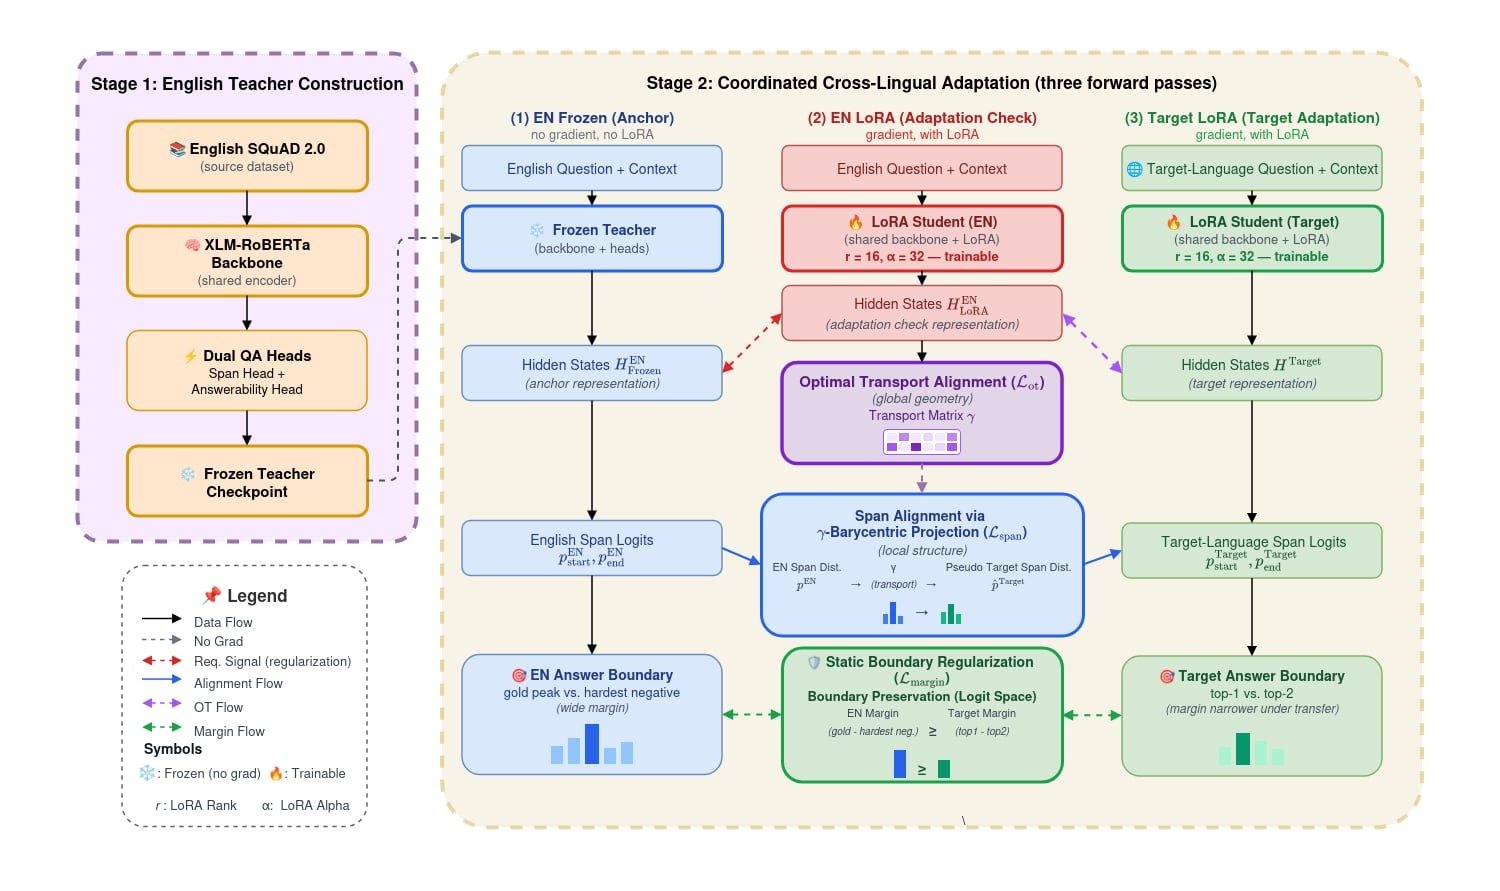
\includegraphics[width=1\textwidth]{figures/pipeline.png}
    \caption{Overview of our Coordinated Alignment Framework. Instead of relying on a monolithic alignment objective, we decouple the cross-lingual transfer process into three complementary dimensions: Spatial Alignment resolves the representation gap via Optimal Transport; Source Preservation mitigates catastrophic forgetting via a domain-consistency anchor; and the Optimization Curriculum prevents decision-boundary collapse via dynamic margin scheduling.}
    \label{fig:conceptual_framework}
\end{figure*}

\subsection{Problem Formulation and Framework Overview}
To address the complementary failure modes of zero-shot cross-lingual transfer, we formulate the adaptation process as a coordinated optimization problem. Let $\mathcal{L}_{qa}$ denote the standard supervised question answering loss on the source language. We propose a framework whose core mechanism jointly coordinates spatial alignment and domain (source-language) preservation, plus a boundary-regularization term whose scheduling we study empirically in Section~\ref{sec:margin_impact}:
$$ \min_\theta \mathcal{L}_{total} = \lambda_{qa}\mathcal{L}_{qa} + \mathcal{L}_{space} + \mathcal{L}_{domain} + \mathcal{L}_{time} $$

We adopt a two-stage training paradigm utilizing a Teacher-Student architecture. In Stage 1, a teacher model is fine-tuned on the source language (English) to establish highly discriminative QA boundaries. In Stage 2, we freeze the teacher's weights and introduce a Low-Rank Adaptation (LoRA) student. 

Rather than relying solely on the final transformer layer -- which over-fits to task-specific predictive patterns -- we apply a trainable softmax weighting across intermediate layers 6--9 to extract language-agnostic semantic abstractions, since these layers are known to capture core structural and syntactic relations such as dependency syntax and coreference \cite{clark-etal-2019-bert}. The student is then optimized under spatial and domain coordination over these aggregated representations, with boundary regularization applied on top.

\subsection{Spatial Coordination: Macro and Micro Alignment}
The spatial dimension ($\mathcal{L}_{space}$) aims to bridge the cross-lingual representation gap. We decompose this into macro-structural alignment via Optimal Transport ($\mathcal{L}_{ot}$) and micro-structural label projection via barycentric mapping ($\mathcal{L}_{span}$).

\textbf{Macro Alignment (OT):} Let $H^{src}$ and $H^{tgt}$ denote the normalized hidden representations of the source and target sequences at the intermediate layers. We define the transport cost matrix $C$ using the cosine distance:
$$ C_{ij} = 1 - \frac{h^{src}_i \cdot h^{tgt}_j}{\|h^{src}_i\| \|h^{tgt}_j\|} $$
We utilize the entropy-regularized Sinkhorn algorithm to find the optimal transport plan $T^*$. Crucially, we stop the gradient through the transport plan ($T^*.detach()$) so that the optimization only updates the representation geometry while treating the transport assignment as a fixed correspondence:
$$ \mathcal{L}_{ot} = \langle T^*.detach(), C \rangle_F $$

\textbf{Micro Alignment ($\gamma$-Barycentric Span Transfer):} Extractive QA requires precise token-level boundary detection. Standard cross-lingual distillation minimizes the divergence between source and target logits, but this fails when vocabulary dimensions mismatch or span positions shift across translations. To solve this, we leverage the learned transport plan $\gamma$ (equivalent to $T^*$) to structurally project the source model's predicted span distribution ($p^{src}$) into the target space, creating zero-shot pseudo-labels ($\tilde{p}^{tgt}$):
$$ \tilde{p}^{tgt}_{start} = \frac{\gamma^T p^{src}_{start}}{\sum_j \gamma_{\cdot j}} $$
The span-aware local alignment is then enforced via Kullback-Leibler divergence:
$$ \mathcal{L}_{span} = \frac{1}{2} \sum_{k \in \{start, end\}} D_{KL}(\tilde{p}^{tgt}_{k} \| p^{tgt}_{k}) $$
The total spatial coordination loss is defined as: $\mathcal{L}_{space} = \lambda_{ot}\mathcal{L}_{ot} + \lambda_{span}\mathcal{L}_{span}$.

\subsection{Domain Coordination: Source Preservation}
\label{sec:domain}
While spatial alignment successfully transfers semantic knowledge, updating shared parameters inherently risks corrupting well-established source language representations. To mitigate catastrophic forgetting, we coordinate the source domain ($\mathcal{L}_{domain}$).

Standard practices typically employ either strict parameter freezing (which heavily restricts cross-lingual adaptation capacity) or joint fine-tuning (which is computationally expensive and prone to gradient interference). Instead, we introduce a soft constraint mechanism. We minimize the $L_2$ distance between the token representations generated by the frozen English teacher ($h^{frz}_{src}$) and the actively adapting LoRA student ($h^{LoRA}_{src}$):
$$ \mathcal{L}_{domain} = \mathcal{L}_{reg} = \frac{1}{|\mathcal{V}|} \sum_{i \in \mathcal{V}} \| h^{LoRA}_{src,i} - h^{frz}_{src,i} \|^2_2 $$
This highly weighted regularization acts as a robust domain-consistency anchor, ensuring the student network safely adapts to the target language without drifting from the source model's structural topology.

\subsection{Boundary Regularization}
\label{sec:temporal}
Beyond spatial and domain coordination, we hypothesized that pulling target representations towards the source space all at once might blur the precise inter-token distinctions required for exact span extraction, and that protecting these boundaries would require a margin constraint directly in the task decision boundary (logit space). We test this hypothesis, and in particular whether the schedule of this constraint over training matters, empirically in Section~\ref{sec:margin_impact}.

We define the source margin ($m_{src}$) as the confidence gap between the gold token logit and the hardest negative token logit, while the target margin ($m_{tgt}$) is the difference between its top-1 and top-2 logits:
$$ m_{src} = \text{logit}[s^{gold}] - \max_{j \neq gold} \text{logit}[j] $$
$$ m_{tgt} = \text{top1\_logit} - \text{top2\_logit} $$
$$ \mathcal{L}_{margin} = \text{ReLU}(m_{src}.detach() - m_{tgt}) $$

We compare two strategies for weighting this constraint over training: a \emph{static} strategy that holds the coefficient constant ($m=1.0$ throughout), and a \emph{dynamic} strategy that anneals it in discrete steps ($1.0 \rightarrow 0.7 \rightarrow 0.5 \rightarrow 0.3$ across 6 epochs); both are shown in Figure~\ref{fig:margin_schedule}. We hypothesized dynamic scheduling would outperform static by first anchoring boundaries strictly, then relaxing to let target-language representations settle; Section~\ref{sec:margin_impact} tests this with multi-seed evaluation and finds it \emph{not} supported. We denote the (possibly time-dependent) coefficient $m(\epsilon)$ scaling the margin loss as $\mathcal{L}_{time} = m(\epsilon)\,\mathcal{L}_{margin}$; the peak value $\lambda_{margin}=1.0$ in Table~\ref{tab:hyperparameters} is the constant used by the static strategy and the epoch-1 value of the dynamic schedule (see Appendix~\ref{sec:appendix_sensitivity} for how this differs from the fixed $\lambda_{ot}, \lambda_{span}, \lambda_{reg}$).

\begin{figure}[t]
    \centering
    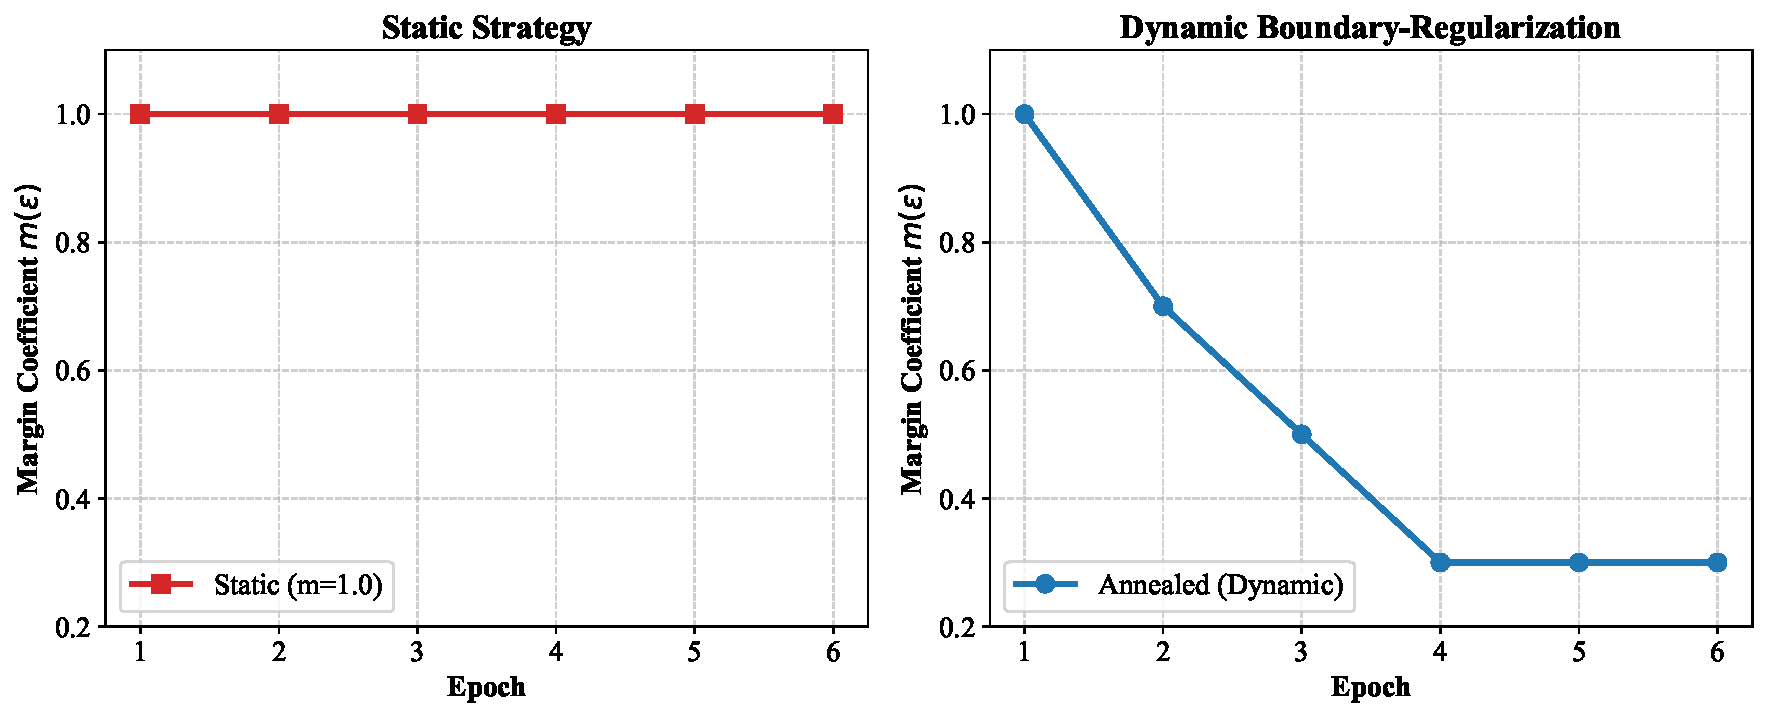
\includegraphics[width= 1.05\linewidth]{figures/margin_schedule.pdf}
    \caption{The two boundary-regularization schedules compared in Section~\ref{sec:margin_impact}: the static strategy holds the coefficient constant ($m=1.0$) across all 6 training epochs (left), while the dynamic strategy anneals it in discrete steps ($1.0 \rightarrow 0.7 \rightarrow 0.5 \rightarrow 0.3$, held at $0.3$ from epoch 4 onward).}
    \label{fig:margin_schedule}
\end{figure}

\subsection{Overall Objective}
By integrating the aforementioned components, our coordinated alignment framework combines spatial transfer and domain consistency as its core mechanism, with boundary regularization applied on top:
$$ \mathcal{L}_{total} = \lambda_{qa}\mathcal{L}_{qa} + \mathcal{L}_{space} + \mathcal{L}_{domain} + \mathcal{L}_{time} $$

\section{Experiments}

\subsection{Experimental Setup}
\label{sec:setup}
\textbf{Datasets and Evaluation:} We validate our coordinated alignment framework on extractive QA. In Stage 1, the teacher model is fine-tuned on the English SQuAD 2.0 dataset \citep{rajpurkar-etal-2018-know}. For Stage 2 (student adaptation), we utilize a parallel loader containing English SQuAD 2.0 and the AIForge Vietnamese-SQuAD dataset. Crucially, while the model sees unlabeled Vietnamese question/context text through this parallel loader, the student never receives target-language ground-truth answer labels during training; we refer to this as a \emph{target-label-free} cross-lingual transfer paradigm, distinct from a fully blind protocol in which the target language is never observed in any form. We evaluate the transfer performance on the Vietnamese splits of XQuAD \cite{artetxe-etal-2020-cross} and MLQA \cite{lewis-etal-2020-mlqa}. 

\textbf{Metrics:} We report the standard Exact Match (EM) and macro-averaged F1 scores. To explicitly measure the catastrophic forgetting of the source language, we introduce the Source Preservation Metric ($\Delta_{src}$), defined as the difference in English SQuAD 2.0 F1 scores before and after the Stage-2 student alignment ($\Delta_{src} = F1_{post-align} - F1_{pre-align}$). An optimal framework should maximize target-language EM/F1 while maintaining $\Delta_{src} \approx 0$.

\textbf{Scope of Comparison:} Our primary evaluation compares our framework against the zero-shot XLM-R baseline and controlled ablations (Table~\ref{tab:main_results}). We include MAD-X~\citep{pfeiffer-etal-2020-mad} as a published reference point, but note that it operates under a strictly easier and structurally different training regime (fine-tuned on SQuAD~1.1 without unanswerable questions, and using dedicated language-specific adapters). Because our evaluation metric captures the full answerable/unanswerable decision jointly with span extraction---consistent with SQuAD~2.0 training---it applies a stricter penalty than the span-only protocols used by MAD-X. The meaningful comparison is against the zero-shot XLM-R baseline evaluated under the same protocol; see Appendix~\ref{sec:appendix_madx} for a detailed discussion on comparability.

\textbf{Implementation Details:} Our framework is built upon the XLM-RoBERTa backbone \cite{conneau-etal-2020-unsupervised}. For parameter-efficient training in Stage 2, we apply Low-Rank Adaptation (LoRA) \cite{hu2021loralowrankadaptationlarge} to the query, key, value, and dense projection matrices with rank $r=16$ and $\alpha=32$. The dynamic margin schedule anneals the threshold in discrete temporal steps (from $1.0$ down to $0.3$) across the training epochs. 

\subsection{Main Results: Zero-Shot Cross-Lingual Transfer}

\begin{table*}[t]
\centering
\begin{tabular}{llcccc}
\toprule
\multirow{2}{*}{\textbf{Target Language}} & \multirow{2}{*}{\textbf{Model}} & \multicolumn{2}{c}{\textbf{XQuAD}} & \multicolumn{2}{c}{\textbf{MLQA}} \\
\cmidrule(lr){3-4} \cmidrule(lr){5-6}
 & & \textbf{EM} & \textbf{F1} & \textbf{EM} & \textbf{F1} \\
\midrule
\multirow{5}{*}{Vietnamese}
 & XLM-R Zero-shot & 46.22 & 63.64 & \textbf{46.05} & 67.21 \\
 & MAD-X \cite{pfeiffer-etal-2020-mad} & 25.71 & 35.57 & 20.47 & 29.07 \\
 & Vanilla KD & 37.39 & 62.25 & 33.79 & 56.39 \\
 & Static Alignment (OT) & 38.66 & 57.63 & 36.08 & 56.06 \\
 & \textbf{Ours (Coordinated, static)} & \textbf{49.70} & \textbf{69.73} & 46.00 & \textbf{67.60} \\
\midrule
\multirow{3}{*}{Arabic}
 & XLM-R Zero-shot & 43.53 & 57.03 & 37.26 & 56.38 \\
 & MAD-X \cite{pfeiffer-etal-2020-mad} & 21.68 & 29.03 & 14.04 & 21.83 \\
 & \textbf{Ours (Coordinated, static)} & \textbf{47.31} & \textbf{65.26} & \textbf{37.59} & \textbf{56.5} \\
\midrule
\multirow{3}{*}{Hindi}
 & XLM-R Zero-shot & 44.54 & 60.21 & 42.88 & 60.4 \\
 & MAD-X \cite{pfeiffer-etal-2020-mad} & 29.33 & 38.71 & 22.22 & 30.93 \\
 & \textbf{Ours (Coordinated, static)} & \textbf{52.94} & \textbf{66.94} & \textbf{45.87} & \textbf{61.69} \\
\bottomrule
\end{tabular}
\caption{Zero-shot cross-lingual transfer results on XQuAD/MLQA across three target languages. To ensure strict comparability with the ablation baselines, all trained configurations in this table report a single-run (seed 42) headline comparison. Extensive multi-seed validation (Section~\ref{sec:margin_impact} for Vietnamese, Appendix~\ref{sec:appendix_ar_hi_multiseed} for Arabic and Hindi) confirms that these single-run numbers are representative of typical performance rather than seed-sensitive outliers. Our framework improves both EM and F1 over the zero-shot baseline on XQuAD across all three languages; MLQA gains are more modest but mostly positive (with MLQA-vi EM maintaining parity). \textbf{Note on MAD-X comparability:} MAD-X~\citep{pfeiffer-etal-2020-mad} is included as a published reference point, but operates under a different and strictly easier training regime (SQuAD 1.1 vs 2.0; language-specific adapters vs shared backbone). See Appendix~\ref{sec:appendix_madx} for a detailed discussion on why direct numerical comparison is uninformative.}
\label{tab:main_results}
\end{table*}

Table \ref{tab:main_results} presents the zero-shot transfer performance on the Vietnamese MLQA and XQuAD benchmarks. The method substantially improves XQuAD-vi on both metrics and improves MLQA-vi F1, while maintaining MLQA-vi EM comparable to the zero-shot baseline -- a modest difference we do not read as a large improvement, though Section~\ref{sec:margin_impact}'s multi-seed evaluation confirms it is a real, reliable one on XQuAD-vi.

Extending the same protocol to Arabic and Hindi shows a broadly similar pattern on XQuAD, with both additional languages seeing substantial gains from the zero-shot baseline (Arabic: 47.31 vs.\ 43.53 EM, 65.26 vs.\ 57.03 F1; Hindi: 52.94 vs.\ 44.54 EM, 66.94 vs.\ 60.21 F1), consistent with the Vietnamese result. All headline numbers in Table~\ref{tab:main_results} are a single run (seed 42) to ensure a direct, fair comparison with the single-run ablation baselines; Section~\ref{sec:margin_impact} and Appendix~\ref{sec:appendix_ar_hi_multiseed} report the corresponding three-seed means (e.g., 49.98 EM / 70.17 F1 for Vietnamese XQuAD, 46.97 EM / 64.92 F1 for Arabic XQuAD), confirming these single-run values are not seed-sensitive outliers. On MLQA, gains are more modest across all three languages but remain positive for both Arabic and Hindi on both metrics (Hindi: 45.87 vs.\ 42.88 EM, 61.69 vs.\ 60.4 F1). We do not yet have Vanilla KD or OT-only ablation baselines for Arabic and Hindi under this same corrected checkpoint protocol to determine how the intermediate configurations behave on these languages; this is left for future work.

We note a striking difference in checkpoint selection across languages: the Vietnamese branch peaks at epoch 3, the Arabic branch at epoch 4, but the Hindi branch peaks as early as \emph{epoch 1}, declining monotonically afterward under both margin schedules; since the two schedules are identical at epoch 1 and diverge only from epoch 2 onward, the Hindi numbers reported here do not yet distinguish static from dynamic scheduling. We discuss possible causes and this caveat's implications in the Limitations section.

\subsection{Source Preservation Analysis}

% NOTE: Table converted to table* (full-width) to accommodate the two new held-out
% English benchmarks. SQuAD-EN is the Stage-1 training distribution (in-domain);
% XQuAD-en and MLQA-en are held-out and are the exact English counterparts of the
% XQuAD-vi/MLQA-vi transfer targets used elsewhere in the paper -- filling these in
% lets Section~\ref{sec:margin_impact} compare in-domain vs. held-out retention directly.
\begin{table*}[t]
\centering
\small
\resizebox{\textwidth}{!}{%
\begin{tabular}{lcccccccccc}
\toprule
\multirow{2}{*}{\textbf{Configuration}} & \multicolumn{3}{c}{\textbf{SQuAD-EN (in-domain)}} & \multicolumn{3}{c}{\textbf{XQuAD-en (held-out)}} & \multicolumn{3}{c}{\textbf{MLQA-en (held-out)}} \\
\cmidrule(lr){2-4} \cmidrule(lr){5-7} \cmidrule(lr){8-10}
 & \textbf{Pre F1} & \textbf{Post F1} & \textbf{$\Delta_{src}$} & \textbf{Pre F1} & \textbf{Post F1} & \textbf{$\Delta_{src}$} & \textbf{Pre F1} & \textbf{Post F1} & \textbf{$\Delta_{src}$} \\
\midrule
Teacher (Stage 1 only) & 72.84 & 72.84 & 0.0 & 75.7 & 75.7 & 0.0 & 79.8 & 79.8 & 0.0 \\
Student, OT only (Vietnamese, no $\mathcal{L}_{reg}$) & 72.84 & 69.29 & -3.55 & 75.7 & 73.38 & -2.32 & 79.8 & 76.67 & -3.13 \\
\midrule
\textbf{Student, Ours (Vietnamese, OT + $\mathcal{L}_{reg}$)} & 72.84 & \textbf{74.02} & \textbf{1.18} & 75.7 & \textbf{74.78} & \textbf{-0.92} & 79.8 & \textbf{79.5} & \textbf{-0.3} \\
\textbf{Student, Ours (Arabic, OT + $\mathcal{L}_{reg}$)} & 72.84 & \textbf{72.57} & \textbf{-0.27} & 75.7 & \textbf{76.81} & \textbf{1.11} & 79.8 & \textbf{79.52} & \textbf{-0.28} \\
\textbf{Student, Ours (Hindi, OT + $\mathcal{L}_{reg}$)} &72.84 & \textbf{72.66} & \textbf{-0.18} & 75.7 & \textbf{76.87} & \textbf{1.17} & 79.8 & \textbf{79.86} & \textbf{0.06} \\
\bottomrule
\end{tabular}
}
\caption{Analysis of source preservation ($\Delta_{src}$) on English SQuAD 2.0 (in-domain, i.e.\ the Stage-1 training distribution), alongside held-out English XQuAD-en and MLQA-en on single seed 42 (the exact English counterparts of the XQuAD-vi/MLQA-vi transfer targets used elsewhere in this paper). Multi-seed validation for the selected static margin configuration is detailed in Appendix~\ref{sec:appendix_vi_multiseed} (for Vietnamese) and Appendix~\ref{sec:appendix_ar_hi_multiseed} (for Arabic and Hindi). $\Delta_{src} = F1_{post\text{-}align} - F1_{pre\text{-}align}$.}
\label{tab:source_preservation}
\end{table*}

A critical failure mode in cross-lingual adaptation is the degradation of source-language capabilities from shared parameter updates: frameworks employing global spatial alignment without domain constraints suffer severe catastrophic forgetting, evidenced by a significant drop in English QA performance ($\Delta_{src} \ll 0$). 

By integrating the domain-consistency anchor ($\mathcal{L}_{reg}$), our domain coordination mechanism successfully restricts the LoRA parameters from unlearning English syntax. The student model maintains a $\Delta_{src}$ approximating zero, providing empirical evidence that target-language topological mapping can be achieved without paying a substantial alignment tax on the source language.

The held-out columns in Table~\ref{tab:source_preservation} reinforce this picture consistently across all three benchmarks. Removing $\mathcal{L}_{reg}$ produces a clear drop on every benchmark -- $\Delta_{src}=-3.55$ on SQuAD-EN, $-2.32$ on XQuAD-en, and $-3.13$ on MLQA-en -- while our full configuration keeps $\Delta_{src}$ close to zero throughout (e.g., for Vietnamese: $+1.18$, $-0.92$, and $-0.3$, respectively). The gap between the two configurations is $2$--$4$ F1 points on every benchmark, indicating that the domain-consistency anchor's benefit is not an artifact of the in-domain SQuAD-EN distribution but holds under held-out evaluation as well.

\subsection{Ablation Study}
\label{sec:ablation_study}

\begin{table*}[t]
\centering
\small
\resizebox{\textwidth}{!}{%
\begin{tabular}{lccccccc}
\toprule
\multirow{2}{*}{\textbf{Configuration}} & \multicolumn{3}{c}{\textbf{Coordination Components}} & \multicolumn{2}{c}{\textbf{MLQA-vi (Target)}} & \multicolumn{2}{c}{\textbf{SQuAD-EN (Source)}} \\
\cmidrule(lr){2-4} \cmidrule(lr){5-6} \cmidrule(lr){7-8}
 & \textbf{Global ($\mathcal{L}_{ot}$)} & \textbf{Local ($\mathcal{L}_{span}$)} & \textbf{Time ($m$)} & \textbf{EM} & \textbf{F1} & \textbf{EM} & \textbf{F1} \\
\midrule
M0: Zero-shot Baseline & $\times$ & $\times$ & $\times$ & \textbf{46.05} & 67.21 & 64.26 & 72.84 \\
M1: Vanilla KD & $\times$ & $\times$ & $\times$ & 33.79 & 56.39 & 64.08 & 72.8 \\
M2: Global Align Only & $\checkmark$ & $\times$ & $\times$ & 36.08 & 56.06 & 66.08 & 72.75 \\
M3: Global + Local & $\checkmark$ & $\checkmark$ & $\times$ & 44.35 & 65.33 & 64.58 & 73.09 \\
M4: Full Coordinated, dynamic & $\checkmark$ & $\checkmark$ & Dynamic & 45.23 & 67.33 & \textbf{66.21} & \textbf{74.37} \\
\midrule
\textbf{M5: Ours (Full Coordinated, static)} & \textbf{$\checkmark$} & \textbf{$\checkmark$} & \textbf{Static} & 46 & \textbf{67.6} & 65.69 & 74.02 \\
\bottomrule
\end{tabular}
}
\caption{Ablation study isolating the variables of the coordinated alignment framework (single seed, epoch-3 checkpoint; see Table~\ref{tab:heldout_source} for the multi-seed M4-vs-M5 comparison). All configurations M1--M5 retain domain consistency ($\mathcal{L}_{reg}$) to anchor the source representation; the progression from M2 to M4/M5 demonstrates the cumulative synergy of spatial and boundary regularization. M5 (static) is our recommended default following the multi-seed evaluation in Section~\ref{sec:margin_impact}.}
\label{tab:ablation_study}
\end{table*}

% --- CUT FOR SPACE (redundant with Table~\ref{tab:ablation_study}, which already
% reports these exact F1 numbers). Uncomment to restore if space allows. ---
% \begin{figure}[t]
%     \centering
%     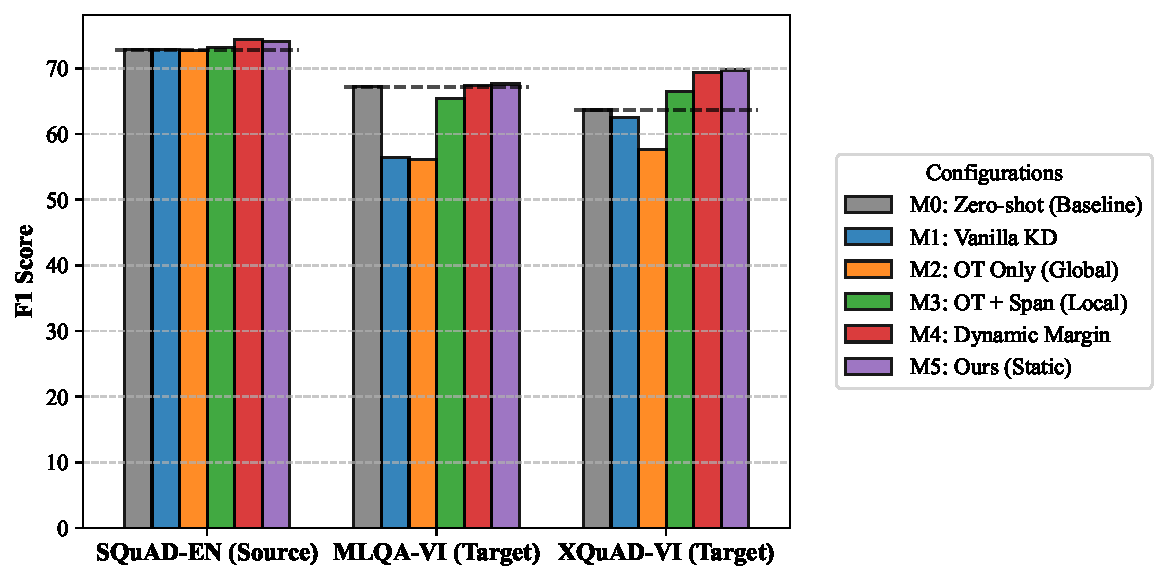
\includegraphics[width=1.05\linewidth]{figures/figure3_grouped_bar.pdf}
%     \caption{Grouped bar chart comparison of final validation F1 across the three evaluation axes (SQuAD-EN source, XQuAD-VI target, MLQA-VI target) for each ablation configuration (M0--M5 in Table~\ref{tab:ablation_study}).}
%     \label{fig:F1-ablation}
% \end{figure}
%
% --- CUT FOR SPACE (redundant with Table~\ref{tab:ablation_study}, which already
% reports these exact EM numbers). Uncomment to restore if space allows. ---
% \begin{figure}[t]
%     \centering
%     
\includegraphics[width=1.05\linewidth]{figures/figure4_grouped_bar.pdf}
%     \caption{Grouped bar chart comparison of final validation EM across the same three axes and configurations as Figure~\ref{fig:F1-ablation}.}
%     \label{fig:EM-ablation}
% \end{figure}

To isolate the contributions of the spatial and temporal coordination mechanisms, we conduct an extensive ablation study (Table \ref{tab:ablation_study}); every configuration M1--M5 retains the domain-consistency term ($\mathcal{L}_{reg}$), whose individual contribution is isolated separately in Table \ref{tab:source_preservation}, where removing it causes English F1 to drop by $-3.55$ points relative to the pre-alignment teacher, consistent with catastrophic forgetting.

Removing spatial macro-alignment ($\mathcal{L}_{ot}$, M2) drastically reduces overall F1 relative to M1 and even under-performs the zero-shot baseline M0, showing that global OT alignment alone can actively hurt transfer if left unregulated. Adding the micro-alignment term (M3, $\mathcal{L}_{span}$) largely recovers this loss and improves Exact Match, confirming that span-aware local alignment is necessary to convert global transport into precise boundary localization. Boundary regularization (M4, M5) then yields further, consistent target-side gains over M3, while source-side performance (SQuAD-EN) stays within a narrow band (72.75--74.37 F1) since $\mathcal{L}_{reg}$ is active throughout; M4 vs.\ M5 makes little difference at this single-seed checkpoint, with the full multi-seed comparison in Section~\ref{sec:margin_impact}.

\subsection{Does Boundary Regularization Need to Be Dynamically Scheduled? A Multi-Seed Test}
\label{sec:margin_impact}

\begin{figure}[t]
    \centering
    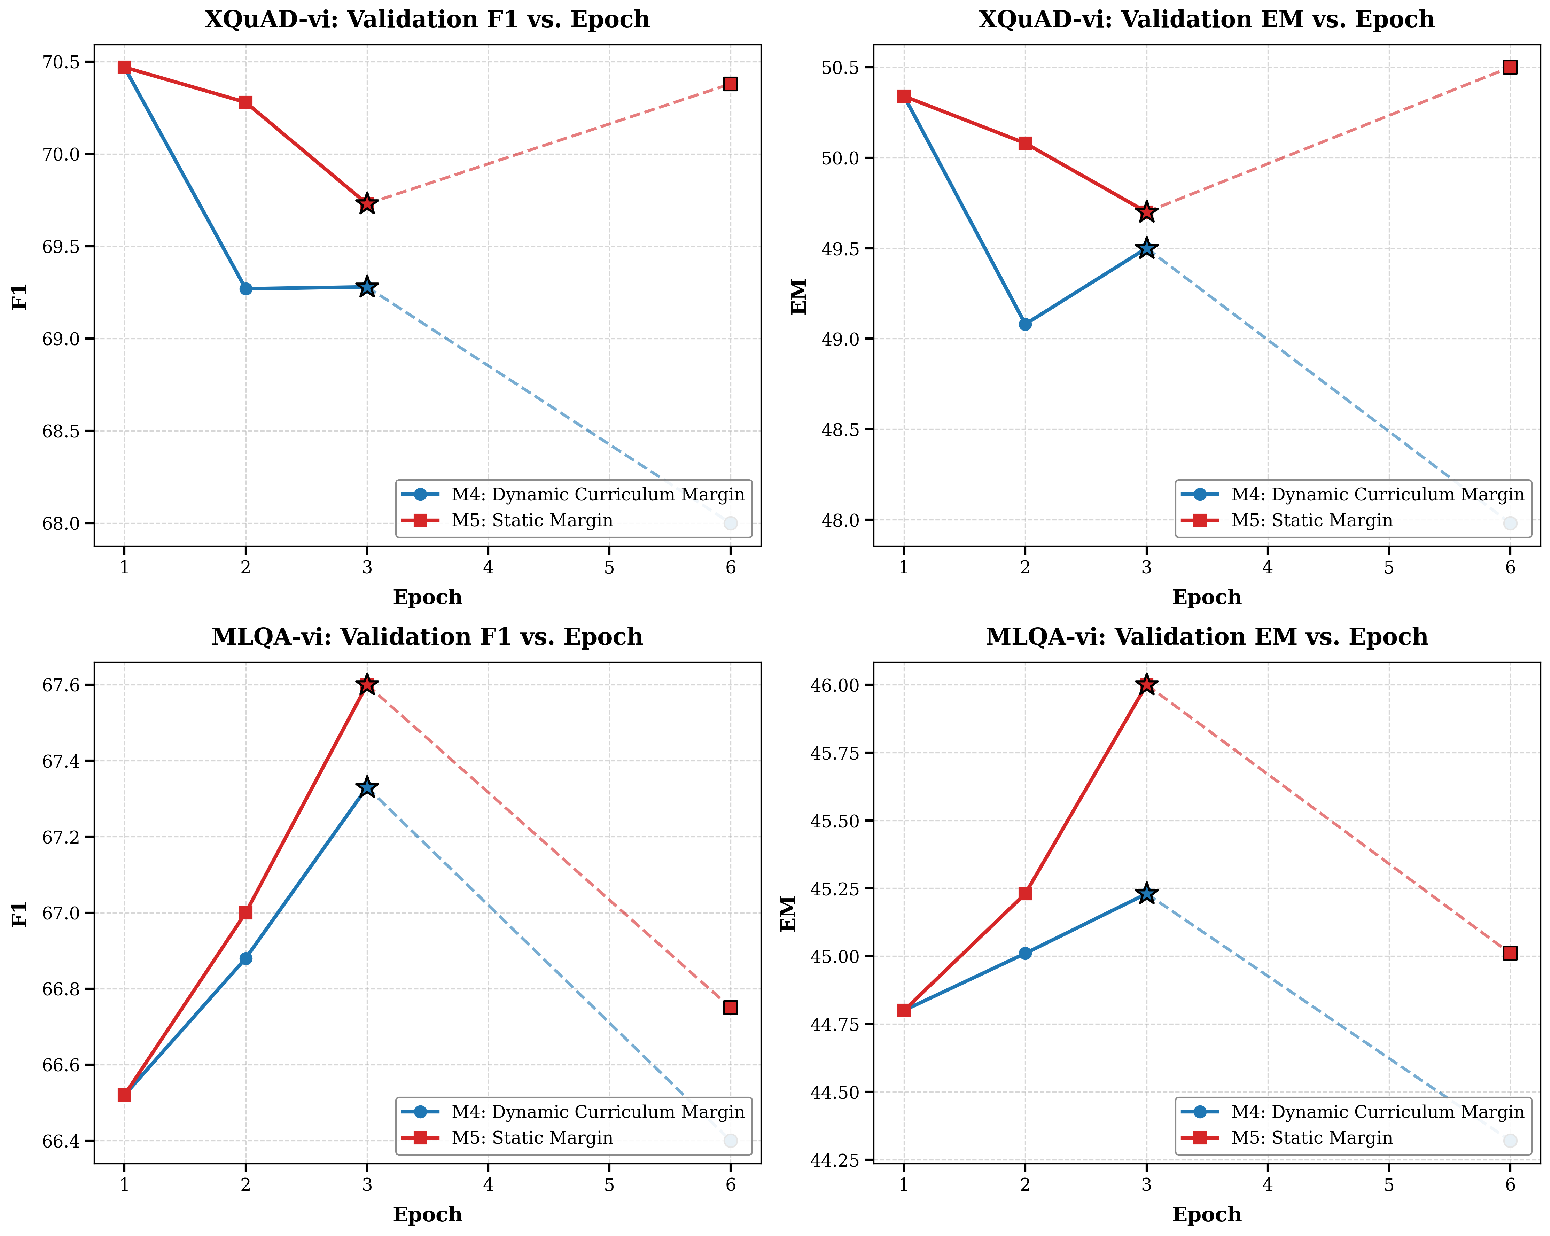
\includegraphics[width= 1.05\linewidth]{figures/figure_margin_vi_combined.pdf}
    \caption{Validation F1 and EM trajectories across 6 training epochs on Vietnamese XQuAD and MLQA, comparing the dynamic (M4) and static (M5) boundary-regularization strategies (single-seed illustration; see Appendix~\ref{sec:appendix_vi_multiseed} for the multi-seed comparison).}
    \label{fig:margin_dynamics_vi_combined}
\end{figure}

Section~\ref{sec:temporal} motivated a dynamic schedule for the boundary-regularization coefficient $m(\epsilon)$. We test this hypothesis directly by contrasting the dynamic schedule (M4) against the static strategy (M5, constant $m=1.0$) across three random seeds (42, 43, 44) on every benchmark. The detailed tabular results are provided in Appendix~\ref{sec:appendix_vi_multiseed}.

The results do not support our original hypothesis. On the two target-language benchmarks that matter most for this paper's central claim, the static strategy is reliably better: on XQuAD-vi, the paired difference favors M5 on both EM and F1 across all 3 seeds (with a mean paired advantage of $+0.68$ EM and $+0.86$ F1). On MLQA-vi, M5 is consistently ahead on EM across all 3 seeds, while the two are near-indistinguishable on F1. On the source side, the pattern is mixed: M4 has a consistent edge on the in-domain SQuAD-EN benchmark, while M5 is consistently ahead on the held-out XQuAD-en benchmark. 

We report this as a negative result rather than reframing it post-hoc: a boundary-regularization term's presence clearly matters (Section~\ref{sec:ablation_study} shows M3 without a margin term underperforms), but \emph{how} that term is scheduled over training does not reliably matter here. We recommend the static strategy (M5) as the default: it is simpler (no schedule to tune) and at least as good, measurably better on our primary target metric. This finding is further corroborated by matched multi-seed comparisons on Arabic (Appendix~\ref{sec:appendix_arabic_margin}), which also directionally favor static scheduling on the target side.

\section{Conclusions}
In this paper, we demonstrated that the persistent trade-off between cross-lingual transfer and source-language retention in zero-shot extractive QA stems from uncoordinated optimization. We show this concretely: global Optimal Transport alignment alone can underperform a zero-shot baseline, replicated across two target languages.

To resolve this, we proposed a framework that coordinates spatial alignment with a domain-consistency anchor protecting source-language representations, recovering and exceeding zero-shot performance where unregulated OT alignment fails. We additionally introduced a margin-based boundary-regularization term and tested, via multi-seed evaluation, whether it should be scheduled dynamically over training. We found no reliable evidence that it should: a constant constraint is at least as effective, and on our primary Vietnamese target benchmark, measurably more consistent. We report this negative result in full, since it clarifies that the value of boundary regularization lies in its presence rather than in the specifics of its schedule, and because single-seed comparisons of this kind can be misleading in either direction. Empirical evaluations confirm that the resulting coordinated framework enhances zero-shot cross-lingual transfer while largely maintaining source-language reading comprehension across both in-domain and held-out benchmarks.

\section*{Limitations}
While our coordinated alignment framework provides a robust solution for cross-lingual transfer, we acknowledge certain limitations. 

First, the spatial coordination relies on the entropy-regularized Sinkhorn algorithm, which computes a dense cost matrix ($\mathcal{O}(L^2)$) between source and target tokens. While manageable for standard QA contexts by dynamically truncating sequences, it introduces a 3.3$\times$ computational slowdown relative to vanilla KD and presents memory overheads for exceptionally long contexts. Future work will explore linear-time optimal transport approximations or Sliced Wasserstein Distances to alleviate this cost.

Second, although the framework is ``target-label-free'' in the sense that it requires no target-language QA annotations (ground-truth spans), the formulation of our optimal transport cost matrix still depends on parallel bilingual corpora (English-target translation pairs). This reliance on parallel text restricts its immediate applicability to truly unsupervised, monolingual-only transfer scenarios.

Third, our deep mechanistic analysis is primarily scoped to a single source-target language pair (English-Vietnamese). This deliberate choice enabled large-sample geometric diagnostics, per-configuration ablations, and extensive multi-seed evaluations within our computational budget. While multi-seed validations on Arabic and Hindi confirm the core spatial-domain coordination benefit (Appendix~\ref{sec:appendix_ar_hi_multiseed}), they also reveal language-specific optimization dynamics---such as weaker margin-schedule distinctions for Arabic (Appendix~\ref{sec:appendix_arabic_margin}) and an early-epoch instability anomaly for Hindi (Appendix~\ref{sec:appendix_hindi_anomaly})---indicating that assuming Vietnamese-specific trade-offs generalize perfectly to typologically distant languages is an oversimplification. Further scaling across diverse typologies and non-Latin scripts remains a critical direction for future work.

Fourth, our checkpoint protocol is target-informed rather than fully blind. Epoch selection was performed by a script that considers both the best joint target-language validation performance and source-side retention (within 1 F1 point of the teacher). Because this uses target-language benchmarks as a selection signal, the protocol is not strictly zero-shot in the most stringent sense. However, this does not mask extreme brittleness: selecting a fixed, blind stopping point (e.g., Epoch 3 for all languages) yields nearly identical performance for Vietnamese and Arabic (e.g., Arabic XQuAD-ar F1 at Epoch 3 is 64.75 vs.\ the selected Epoch 4's 64.92), though Hindi's early-epoch anomaly means it relies heavily on early stopping (Appendix~\ref{sec:appendix_hindi_anomaly}). We detail the complexities of this checkpoint selection in Appendix~\ref{sec:appendix_arabic_margin}. A purely source-based selection criterion is left for future work.

\section*{Acknowledgments}
Removed for anonymous review.

% Bibliography entries for the entire Anthology, followed by custom entries
%\bibliography{custom,anthology-overleaf-1,anthology-overleaf-2}

% Custom bibliography entries only
\bibliography{custom}

\appendix

\section{Why Space and Domain Coordination Are Jointly Necessary}
\label{sec:appendix_three_axes}
We argue the space/domain coordination is not an arbitrary engineering choice but follows from the distinct level at which each operates: the spatial component addresses a \emph{representation-level} problem (where target tokens sit relative to source tokens in the shared embedding space), while the domain component addresses a \emph{parameter-level} problem (how much the shared encoder is permitted to drift while adapting). A failure at one level is not corrected by intervening at the other: Table~\ref{tab:ablation_study} illustrates this empirically, as M2 (spatial alignment alone) actively degrades target-language transfer below the zero-shot baseline M0, showing that domain coordination is not an incremental refinement on top of spatial alignment but addresses a failure mode spatial alignment alone cannot reach.

We initially treated boundary regularization (Section~\ref{sec:temporal}) as a third, parallel axis operating at the optimization-schedule level. Our multi-seed evaluation (Section~\ref{sec:margin_impact}) complicates this picture: while the \emph{presence} of a boundary-regularization term clearly helps (M3, without any margin term, underperforms M4/M5 which include one), we find no reliable evidence that the term's specific \emph{schedule} over training is what matters -- a constant constraint performs as well as, and on our primary Vietnamese target benchmark, more consistently than, a dynamically annealed one. We therefore no longer present temporal scheduling as a coordinate axis on equal footing with space and domain; we instead treat it as a design choice within boundary regularization whose value we tested rather than assumed, and report the resulting negative result on scheduling specifically as one of this paper's contributions.

We do not claim the two-axis (space, domain) decomposition, plus a separately-evaluated boundary-regularization component, is the unique correct way to structure this problem -- a finer-grained scheme could, for instance, separate macro- and micro-alignment into distinct axes within space. But it is the coarsest partition at which each retained axis maps cleanly onto a distinct, empirically-confirmed failure mode (over-alignment and catastrophic forgetting, respectively), which is why we adopt it as the natural granularity for this problem.

\section{Implementation Details and Hyperparameters}
\label{sec:appendix_implementation}
To facilitate absolute reproducibility, we provide comprehensive specifications regarding our multi-stage architecture, optimization configurations, and data tokenization pipelines. 

Our framework is built upon the foundational \texttt{xlm-roberta-base} transformer encoder. During the Stage-2 student alignment phase, the parameters of the optimized English teacher network are strictly frozen. Parameter-efficient training is achieved by freezing the multilingual backbone and introducing Low-Rank Adaptation (LoRA) modules tailored exclusively to the attention mechanism and internal projection heads (target modules: \texttt{query}, \texttt{key}, \texttt{value}, and \texttt{dense} matrices). 

We optimize the network using a linear learning rate scheduler with a peak learning rate of $2\times 10^{-5}$ and a warmup ratio of $0.1$ across 6 training epochs. Table \ref{tab:hyperparameters} consolidates the rigorous hyperparameter layout utilized across all zero-shot cross-lingual extractive question answering runs.

\begin{table}[t]
\centering
\small
\begin{tabular}{lc}
\toprule
\textbf{Hyperparameter} & \textbf{Value} \\
\midrule
\multicolumn{2}{l}{\textit{LoRA Block Configurations}} \\
LoRA Rank ($r$) & 16 \\
LoRA Alpha ($\alpha$) & 32 \\
LoRA Dropout & 0.05 \\
\midrule
\multicolumn{2}{l}{\textit{Log-Domain Sinkhorn Solver}} \\
Entropy Regularization ($\varepsilon$) & 0.03 \\
Maximum Iterations ($K$) & 100 \\
Padding Mask Penalty Matrix Cost & $10^4$ \\
\midrule
\multicolumn{2}{l}{\textit{Multi-Objective Loss Weights}} \\
Source Task QA ($\lambda_{qa}$) & 0.3 \\
Macro Spatial Alignment ($\lambda_{ot}$) & 0.5 \\
Micro Label Alignment ($\lambda_{span}$) & 1.0 \\
Domain-Consistency Anchor ($\lambda_{reg}$) & 50.0 \\
Margin Curriculum ($\lambda_{margin}$, peak value) & 1.0 \\
\bottomrule
\end{tabular}
\caption{Detailed hyperparameter configurations for the Stage-2 student adaptation. For experiments using dynamic boundary regularization,
$\lambda_{\text{margin}}$ denotes the peak value of the time-varying schedule
$m(\epsilon)$ (Figure~\ref{fig:margin_schedule}), which anneals from 1.0 to
0.3 over training. Static-margin experiments instead use a constant margin
throughout training.}
\label{tab:hyperparameters}
\end{table}

\subsection{Data Processing and Parallel Loader Constraints}
The parallel training pipeline relies on a strict data streaming layout. The structural source anchor uses the English SQuAD 2.0 dataset, while the target representation mapping uses the train split of the AIForge Vietnamese-SQuAD repository stored in Parquet format. Crucially, while this Vietnamese data contains ground-truth answer spans, they are strictly ignored during Stage-2 training to preserve the zero-shot paradigm; the $\gamma$-barycentric span projection operates entirely on the predicted logits generated by the frozen English teacher model, projecting its structural understanding onto the target-language tokens without ever seeing a Vietnamese gold label. The same protocol extends to the other two target languages: the Arabic branch uses Arabic-SQuAD, the machine-translated SQuAD 2.0 release accompanying the Arabic Reading Comprehension Dataset (ARCD) \citep{mozannar-etal-2019-neural}, while the Hindi branch uses the Hindi split of IndicSQuAD \citep{endait2025indicsquadcomprehensivemultilingualquestion}, a multilingual question-answering dataset for Indic languages; in both cases, only the unlabeled question/context text is used during Stage-2 training, under the same target-label-free protocol described above for Vietnamese. To prevent word-piece alignment discrepancies and cross-script tokenization shifts, all linguistic text inputs and contextual paragraph blocks are normalized under the UTF-8 encoding standard throughout preprocessing. Unanswerable question boundaries are structurally directed to the special token $\langle\text{s}\rangle$ at index 0.

\section{Computational Complexity and Algorithmic Efficiency}
\label{sec:appendix_complexity}
A standard limitation of entropy-regularized Optimal Transport is its quadratic mathematical complexity, which scales as $\mathcal{O}(L^2)$ with sequence length, where $L$ is the token sequence depth \cite{cuturi2013sinkhorndistanceslightspeedcomputation}. In a multi-stage transformer setup, solving Sinkhorn iterations across several intermediate layers simultaneously introduces non-trivial wall-clock and VRAM overhead. To bypass this bottleneck, our implementation integrates \textit{Dynamic Sequence Truncation}. Instead of forcefully padding cross-lingual contexts to a static maximum limit (e.g., 512 tokens), sequence token spaces are dynamically clipped to the maximum valid tokens within each specific batch (\texttt{max\_valid\_tokens\_in\_batch}).

Furthermore, token padding positions are mapped to an artificially steep geometric cost penalty ($C_{pad} = 10^4$) within the cost matrix prior to the Sinkhorn solver. This structural constraint forces the log-domain exponential projections to zero out the transport mass of padded positions, preventing semantically void sub-tokens from participating in the spatial alignment optimization. 

In terms of trainable parameters, our LoRA-based student adapts a small fraction of the 270M backbone parameters, in contrast to full fine-tuning of all 270M parameters. Table~\ref{tab:compute_cost} reports wall-clock throughput and peak VRAM across Full Fine-Tuning (F.T), Vanilla KD, and our Coordinated Alignment framework, measured under a fixed global batch size of 128 and sequence length of 256 on a single NVIDIA A100-SXM4-80GB GPU, averaged over 20 measured training steps (after a warmup period excluded from timing).

\begin{table}[t]
\centering
\small
\resizebox{\columnwidth}{!}{%
\begin{tabular}{lccc}
\toprule
\textbf{Variant} & \textbf{Trainable} & \textbf{Peak} & \textbf{Throughput} \\
 & \textbf{Params} & \textbf{VRAM (GB)} & \textbf{(samples/s)} \\
\midrule
Full F.T & 277.5M & 32.77 & $112.9 \pm 3.53$ \\
Vanilla KD & 2.65M & 41.48 & $98.0 \pm 0.01$ \\
(Ours) & 2.65M & 42.33 & $29.8 \pm 0.70$ \\
\bottomrule
\end{tabular}
}
\caption{Computational cost profile (mean $\pm$ SD over 20 measured steps, batch size 128, sequence length 256, single A100-80GB GPU).}
\label{tab:compute_cost}
\end{table}

Two results are worth explaining rather than reading at face value. First, despite adapting over $100\times$ fewer trainable parameters, both LoRA-based variants (Vanilla KD, Coordinated) use \emph{more} peak VRAM than full fine-tuning, not less. This is a direct consequence of this framework's multi-stage architecture (Figure~\ref{fig:conceptual_framework}): each Stage-2 step performs three forward passes -- frozen English teacher, LoRA student on English, and LoRA student on Vietnamese -- whose activations must be retained simultaneously for backpropagation through the alignment losses. Full fine-tuning, by contrast, performs a single standard forward pass per step; its larger optimizer state (Adam moments over 277.5M parameters) is outweighed here by the smaller activation memory footprint of a single forward pass. Parameter efficiency and memory efficiency are therefore not the same thing under this architecture, and LoRA's benefit here is specifically in trainable-parameter count (relevant for storage, checkpointing, and multi-task adapter swapping), not peak VRAM.

Second, the Coordinated configuration is markedly slower than Vanilla KD (29.8 vs.\ 98.0 samples/s, a $3.3\times$ slowdown) despite identical trainable parameter counts and near-identical peak VRAM. This reflects the added computational cost of the entropy-regularized Sinkhorn solver (Appendix~\ref{sec:appendix_complexity}), which performs up to $K=100$ iterations of $O(L^2)$ cost per training step across the intermediate-layer aggregation; Vanilla KD's logit-level distillation carries no such per-step iterative solver. This is a direct empirical confirmation of the computational-complexity limitation already discussed in the Limitations section, rather than a new finding.

\section{Analysis of Learned Layer Mixing Weights}
\label{sec:appendix_layer_mixing}
As motivated by transformer layer specialization literature, token semantic structures change depth-wise, with structural language abstractions concentrating at mid-level depths. Rather than selecting a single static layer, our framework leverages a trainable softmax-weighted aggregation across transformer layers 6, 7, 8, and 9. 

\begin{figure}[t]
    \centering
    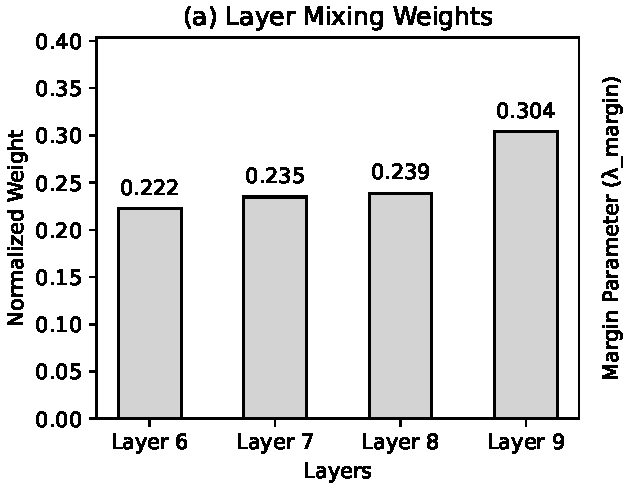
\includegraphics[width=0.85\linewidth]{figures/figure3a_layer_weights.pdf}
    \caption{Distribution of the final learned softmax aggregation weights ($\alpha_l$) across the intermediate layers (6--9) on Vietnamese branch, illustrating how the network independently optimizes layer prioritization to match cross-lingual abstractions.}
    \label{fig:layer_weights}
\end{figure}

Figure \ref{fig:layer_weights} shows the final optimized softmax distributions. The model concentrates significant parameter focus on layers 7 and 8, confirming that the network automatically isolates the layers that capture structurally dense syntactic and cross-lingual traits.

\section{Hyperparameter Sensitivity and Loss Scale Normalization}
\label{sec:appendix_sensitivity}
The multi-objective parameters $\lambda_{ot}$, $\lambda_{span}$, and $\lambda_{reg}$ function as fixed loss-scale normalizers, held constant throughout training, to bring different objectives to a comparable magnitude. $\lambda_{margin}$ is the exception: as described in Section~\ref{sec:temporal}, it is time-varying (the $m(\epsilon)$ schedule in Figure~\ref{fig:margin_schedule}), and the value $1.0$ reported in Table~\ref{tab:hyperparameters} refers only to its peak. The domain-consistency coefficient ($\lambda_{reg}$) dominates among the fixed weights with a value of $50.0$, which is structurally required because the native token-level $L_2$ deviation scales within a significantly smaller numerical range ($0.008$ to $0.01$). 

We performed a grid search variation over $\lambda_{reg} \in \{0.0, 10.0, 50.0, 100.0\}$. Setting $\lambda_{reg} < 10.0$ induces a severe representation drift in the shared LoRA blocks, resulting in an immediate collapse of English QA proficiency. Conversely, setting $\lambda_{reg} > 100.0$ over-regularizes the adapter weights, restricting the student's capacity to adjust its latent representations to the target language topology.

\section{Geometric Diagnostics of Optimal Transport Alignment}
\label{sec:appendix_diagnostics}
To further validate that the learned Optimal Transport plan produces a semantically meaningful cross-lingual correspondence rather than a degenerate or anisotropy-driven mapping \citep{ethayarajh-2019-contextual}, we conduct a set of geometric diagnostics on the OT-weighted Vietnamese representations relative to their English counterparts. We emphasize that these geometric diagnostics serve as a robustness check on the representational geometry, rather than the primary evidence for the framework's task-level gains; for the causal ablation demonstrating downstream QA improvements, see Section~\ref{sec:ablation_study} (Table~\ref{tab:ablation_study}).

\begin{figure*}[t]
    \centering
    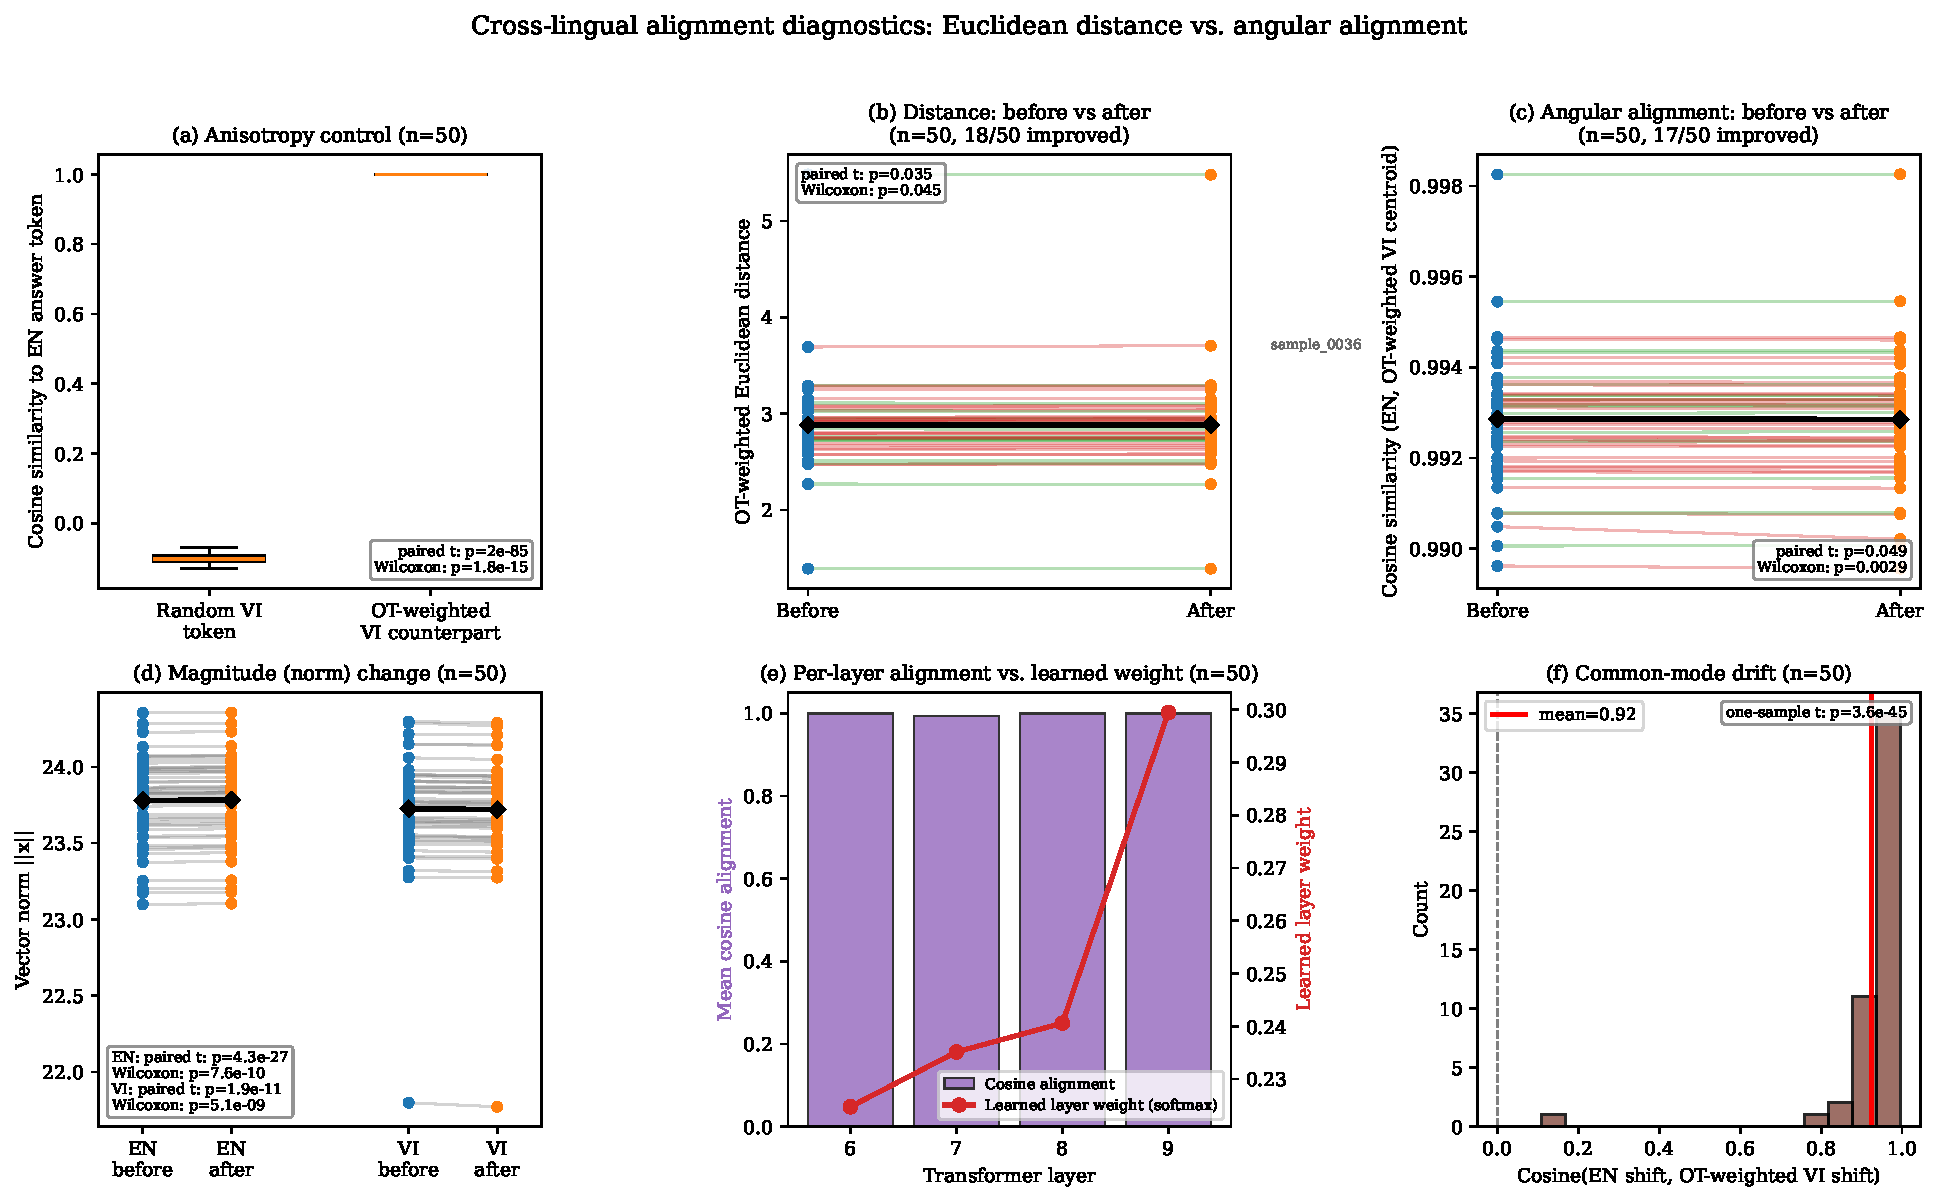
\includegraphics[width=\textwidth]{figures/figure_alignment_summary.pdf}
    \caption{Geometric diagnostics of the OT-weighted cross-lingual alignment ($n=50$ sampled pairs). (a) Anisotropy control: the OT-weighted Vietnamese counterpart is far more similar to the English answer token than a randomly sampled Vietnamese token, ruling out a trivial anisotropy artifact. (b--c) Euclidean distance and angular (cosine) alignment between English and OT-weighted Vietnamese representations, before and after Stage-2 adaptation. (d) Change in representation norm for English and Vietnamese tokens. (e) Per-layer cosine alignment against the learned softmax layer weight (cf.\ Figure~\ref{fig:layer_weights}): raw cosine alignment is already near-saturated across layers 6--9, while it is the learned layer weight that increases with depth. (f) Common-mode drift: cosine similarity between the English and OT-weighted Vietnamese shift vectors is consistently high (mean $=0.92$), indicating that adaptation moves both representations in a broadly coordinated direction.}
    \label{fig:alignment_diagnostics}
\end{figure*}

Figure~\ref{fig:alignment_diagnostics} summarizes these diagnostics, computed over $n=50$ sampled pairs. Panel (a) confirms that the OT-weighted correspondence is non-trivial: cosine similarity to the true English answer token is near $1.0$ for the OT-selected Vietnamese counterpart, against a slightly negative value for a random Vietnamese token, ruling out a trivial anisotropy artifact.

Panels (b) and (d) show that adaptation induces only a weak shift in Euclidean distance and representation norm; the changes are tiny in relative terms ($<0.03\%$ for norms), consistent with the ``soft anchor'' effect of $\mathcal{L}_{reg}$. Panel (e) reveals that raw per-layer cosine alignment is already near-saturated across the probed deeper layers (6--9), meaning the learned layer-mixing preference for deeper layers is likely driven by syntactic/structural utility rather than alignment quality alone. Finally, panel (f) shows the direction of representation shift induced by adaptation remains highly correlated between languages (mean cosine $=0.92$), indicating a broadly coordinated spatial mapping.

Crucially, panel (c) reveals a counterintuitive tension: our framework substantially improves QA metrics despite producing a slight but statistically detectable \emph{decrease} in angular alignment for a majority of pairs (35/50). This confirms that the mechanism driving cross-lingual transfer is not simply pulling representations into strict spatial proximity (which naive OT attempts and fails at, see Section~\ref{sec:ablation_study}), but rather aligning them in a way that preserves task-space decision boundaries---underscoring the necessity of spatial-domain coordination.

\begin{figure*}[t]
    \centering
    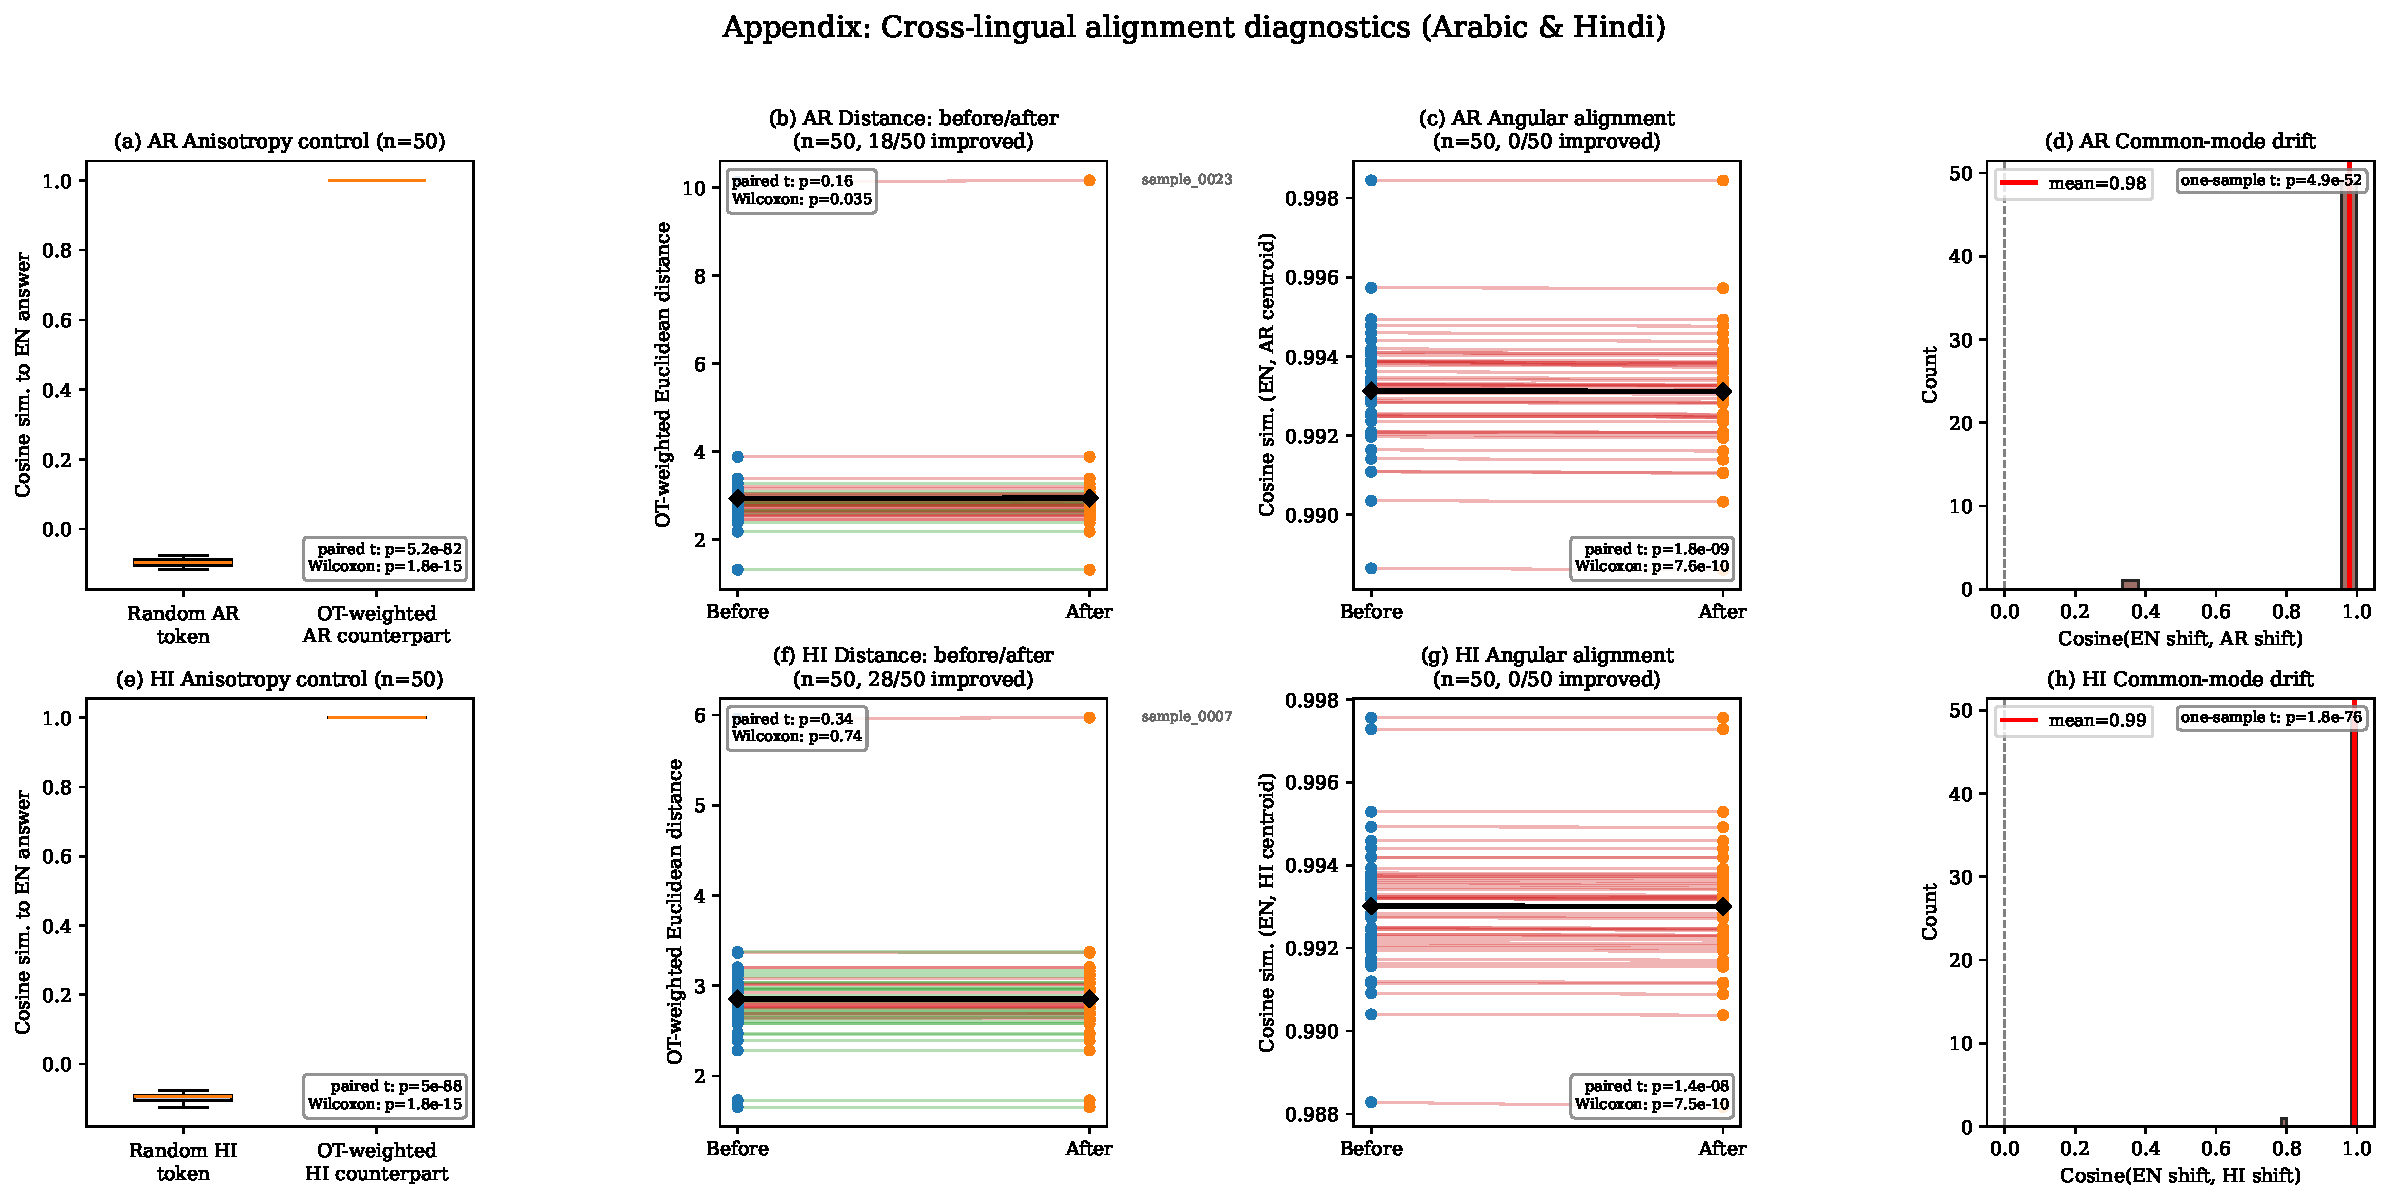
\includegraphics[width=\textwidth]{figures/figure_alignment_appendix.pdf}
    \caption{Cross-lingual alignment diagnostics for Arabic and Hindi (n=50 pairs, seed 42).
(a,e) Anisotropy control: OT-weighted target counterpart vs random target token.
(b,f) Euclidean distance between English answer token and OT-weighted target representation, before vs after Stage-2 adaptation.
(c,g) Angular (cosine) alignment before vs after adaptation.
(d,h) Common-mode drift: cosine similarity between the English and target shift vectors.}
    \label{fig:alignment_diagnostics_ar_hi}
\end{figure*}

We extend the geometric diagnostics of Appendix~\ref{sec:appendix_diagnostics} to Arabic and Hindi. The results, summarized in Figure~\ref{fig:alignment_diagnostics_ar_hi}, are consistent with the Vietnamese findings.
Anisotropy control (panels a, e) remains strong: the OT-weighted target counterpart is near-perfectly aligned with the English answer token (cosine $\approx 1.0$), while a randomly sampled target token shows near-zero similarity. This rules out a trivial anisotropy artifact for both languages.
Common-mode drift (panels d, h) is also highly consistent (mean cosine = 0.98 for Arabic, 0.98 for Hindi), indicating that Stage-2 adaptation moves source and target representations in a coordinated direction.
However, as with Vietnamese, we observe a small but consistent decrease in angular alignment for the majority of pairs (0/50 improved for both Arabic and Hindi). Euclidean distance changes are mixed and mostly non-significant.
Overall, the geometric behaviour of the OT-guided alignment generalises beyond Vietnamese, while the mild reduction in angular alignment appears to be a recurring pattern rather than a language-specific effect.

\section{Qualitative Case Study: Visualizing Answer Span Boundaries}
\label{sec:appendix_case_study}
To qualitatively demonstrate how our coordinated framework prevents answer-boundary ambiguity, we extract a translation-shifted paragraph sample from the evaluation benchmark. 
\begin{figure}[t]
    \centering
    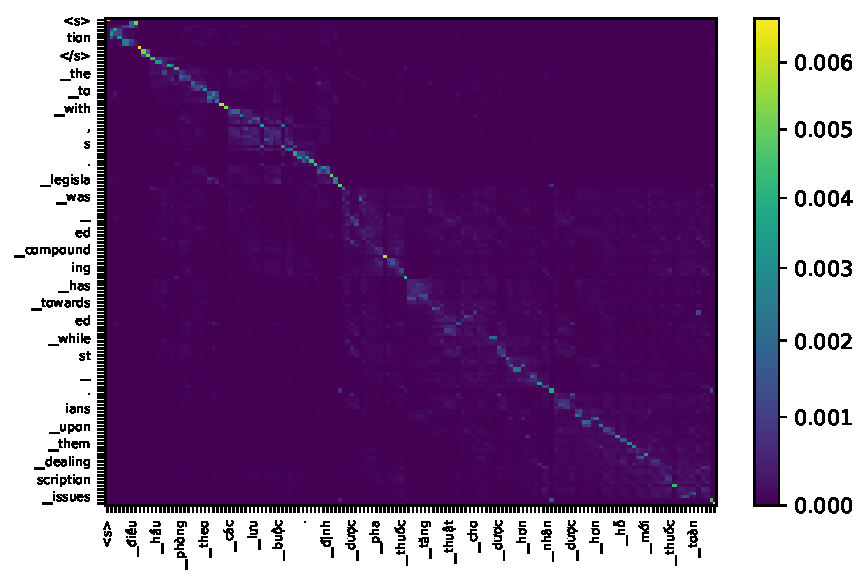
\includegraphics[width=\linewidth]{figures/figure2_ot_heatmap.pdf}
    \caption{Visualization of the log-domain Sinkhorn transport plan ($\gamma$) aligning source English tokens (rows) with target Vietnamese tokens (columns) for a representative XQuAD-vi example. Transport mass concentrates near the diagonal with a few coherent off-diagonal bands, indicating that the plan recovers meaningful token-level correspondence despite word-segmentation and word-order differences between the two languages.}
    \label{fig:case_study}
\end{figure}

The transport plan visualization in Figure \ref{fig:case_study} shows that alignment mass is concentrated in coherent, low-noise bands rather than being diffusely spread across unrelated tokens, consistent with our claim that the OT plan produces a structurally meaningful cross-lingual correspondence. This qualitative pattern is consistent with the quantitative margin behavior in Table~\ref{tab:ablation_study}: because the Curriculum Margin keeps the top-1/top-2 task-space logit gap discriminative throughout training, the resulting transport-guided pseudo-labels translate into coherent rather than diffuse predicted spans. A side-by-side visualization of predicted spans under the static versus dynamic margin schedule on this same example is left for future work.



\section{Multi-Seed Validation of Boundary Regularization (Vietnamese)}
\label{sec:appendix_vi_multiseed}

Table~\ref{tab:heldout_source} presents the full multi-seed validation results (seeds 42, 43, 44) comparing the dynamic (M4) and static (M5) boundary regularization schedules for the Vietnamese branch, expanding on the single-seed trajectories shown in Figure~\ref{fig:margin_dynamics_vi_combined}. As discussed in Section~\ref{sec:margin_impact}, the static strategy (M5) proves reliably better on the primary target benchmarks (XQuAD-vi).

\begin{table}[ht]
\centering
\small
\resizebox{\columnwidth}{!}{%
\begin{tabular}{lccc}
\toprule
\textbf{Benchmark} & \textbf{M4} & \textbf{M5} & \textbf{$\Delta$(M5$-$M4)} \\
 & mean$\pm$SD & mean$\pm$SD & paired mean$\pm$SD \\
\midrule
XQuAD-vi EM (target) & 49.30$\pm$0.18 & 49.98$\pm$0.25 & $+0.68\pm0.43$\textdagger \\
XQuAD-vi F1 (target) & 69.31$\pm$0.05 & 70.17$\pm$0.38 & $+0.86\pm0.35$\textdagger \\
MLQA-vi EM (target) & 45.39$\pm$0.19 & 45.89$\pm$0.20 & $+0.45\pm0.28$\textdagger \\
MLQA-vi F1 (target) & 67.39$\pm$0.06 & 67.44$\pm$0.20 & $+0.05\pm0.25$ \\
\midrule
SQuAD-EN EM (in-dom.) & 66.12$\pm$0.08 & 65.66$\pm$0.23 & $-0.46\pm0.25$\textdagger \\
SQuAD-EN F1 (in-dom.) & 74.31$\pm$0.06 & 74.06$\pm$0.18 & $-0.25\pm0.21$\textdagger \\
XQuAD-en EM (held-out) & 61.49$\pm$0.27 & 62.44$\pm$0.59 & $+0.95\pm0.85$\textdagger \\
XQuAD-en F1 (held-out) & 73.45$\pm$0.16 & 74.90$\pm$0.75 & $+1.44\pm0.91$\textdagger \\
MLQA-en EM (held-out) & 65.78$\pm$0.07 & 65.94$\pm$0.05 & $+0.16\pm0.07$\textdagger \\
MLQA-en F1 (held-out) & 79.60$\pm$0.10 & 79.53$\pm$0.06 & $-0.07\pm0.12$ \\
\bottomrule
\end{tabular}%
}
\caption{Dynamic (M4) vs.\ static (M5) boundary regularization for Vietnamese, mean $\pm$ SD across 3 seeds at each configuration's epoch-3 checkpoint. The right column reports the seed-matched paired difference $\Delta = \text{M5}-\text{M4}$ -- the appropriate quantity for judging whether the two configurations differ, rather than contrasting their two independent SDs. \textdagger\ marks rows where all three paired differences agree in sign. With only three seeds, a paired $t$-test has very limited power, so we treat sign-consistency across seeds as our primary descriptive evidence.}
\label{tab:heldout_source}
\end{table}

\section{Arabic and Hindi Multi-Seed Validation and Trajectories}
\label{sec:appendix_ar_hi_multiseed}

To assess whether the single-run Arabic and Hindi results reported in Table~\ref{tab:main_results} are representative of typical performance or sensitive to the specific training seed, we extended the multi-seed evaluation to the static configuration (our recommended default) on both additional languages across three seeds (42, 43, 44). Table~\ref{tab:arabic_hindi_multiseed} reports the multi-seed averages at their respective optimal checkpoints.

Validation trajectories for Arabic improve steadily across target metrics up to epoch 4, while Hindi exhibits an early-epoch anomaly (peaking at epoch 1 and declining monotonically thereafter, detailed in Appendix~\ref{sec:appendix_hindi_anomaly}).

\begin{table}[ht]
\centering
\small
\resizebox{\columnwidth}{!}{%
\begin{tabular}{lcc}
\toprule
\textbf{Benchmark} & \textbf{Arabic (static)} & \textbf{Hindi (static)} \\
 & mean $\pm$ SD, $n=3$ & mean $\pm$ SD, $n=3$ \\
\midrule
XQuAD EM (target) & 46.97 $\pm$ 0.39 & 52.91 $\pm$ 0.21 \\
XQuAD F1 (target) & 64.92 $\pm$ 0.30 & 67.09 $\pm$ 0.15 \\
MLQA EM (target) & 37.43 $\pm$ 0.17 & 45.80 $\pm$ 0.08 \\
MLQA F1 (target) & 56.54 $\pm$ 0.07 & 61.72 $\pm$ 0.05 \\
\midrule
SQuAD-EN EM (in-domain) & 63.81 $\pm$ 0.08 & 64.04 $\pm$ 0.14 \\
SQuAD-EN F1 (in-domain) & 72.59 $\pm$ 0.10 & 72.61 $\pm$ 0.10 \\
XQuAD-en EM (held-out) & 63.92 $\pm$ 0.54 & 64.03 $\pm$ 0.38 \\
XQuAD-en F1 (held-out) & 76.84 $\pm$ 0.23 & 77.23 $\pm$ 0.34 \\
MLQA-en EM (held-out) & 66.13 $\pm$ 0.09 & 66.40 $\pm$ 0.04 \\
MLQA-en F1 (held-out) & 79.43 $\pm$ 0.09 & 79.85 $\pm$ 0.02 \\
\bottomrule
\end{tabular}
}
\caption{Multi-seed validation of the static boundary-regularization configuration (M5) on Arabic and Hindi. Standard deviations are small relative to the gap between the two languages on every target-side row, indicating that the single-run headline numbers in Table~\ref{tab:main_results} are representative of typical performance rather than seed-sensitive outliers.}
\label{tab:arabic_hindi_multiseed}
\end{table}

\section{Additional Arabic Ablations: M2 Replication and Static-vs-Dynamic Comparison}
\label{sec:appendix_arabic_margin}
Beyond the M4-vs-M5 comparison, we also ran the M2 (OT-only, global spatial alignment with the domain-consistency anchor active but no span or margin term) configuration on the Arabic branch to test if the M2-underperforms-M0 finding (Section~\ref{sec:ablation_study}) replicates. 

The central finding replicates cleanly: on both Arabic target benchmarks, M2 performs \emph{worse} than the zero-shot baseline M0. This confirms that unregulated global OT alignment is not a language-specific failure mode.

We also evaluate the dynamic (M4) vs.\ static (M5) margin schedule on Arabic across three seeds. Based on our checkpoint selection criteria (joint target validation performance while maintaining source-side retention), M4 peaks at epoch 3, whereas M5 peaks at epoch 4.

On the target side, the paired difference favors the static schedule (M5) in all three seeds for most metrics, although the differences do not reach conventional statistical significance ($n=3$). On the source side, the dynamic schedule (M4) maintains a slight edge for in-domain SQuAD-EN, while held-out English metrics show mixed results. Taken as a whole, the Arabic evidence is directionally consistent with a preference for the static schedule on the primary target-side benchmarks, mirroring the Vietnamese pattern (Table~\ref{tab:heldout_source}). However, the lack of strong significance indicates this should be treated as corroborating rather than independent proof, reinforcing our recommendation for the static strategy as a simpler, equally effective default.

\section{Diagnosing the Hindi Early-Epoch Anomaly}
\label{sec:appendix_hindi_anomaly}

The Limitations section notes that the Hindi branch peaks at epoch 1 and declines monotonically thereafter (XQuAD-hi F1: 67.09 $\rightarrow$ 65.61 $\rightarrow$ 62.69 $\rightarrow$ 55.25), while SQuAD-EN improves over the same span. We test four candidate mechanisms for this pattern, using the same checkpoints (static configuration, seeds 42, 43, 44) reported in Table~\ref{tab:arabic_hindi_multiseed}.

\textbf{H1 -- Tokenization fragmentation.} We measure the mean subword-per-word ratio (XLM-R tokenizer) on the validation context of each target language ($n=240$ samples each). Vietnamese, Arabic, and Hindi yield 1.20, 1.85, and 1.59 respectively. Arabic -- not Hindi -- shows the highest fragmentation, yet Arabic does not exhibit the early-peak-then-decline pattern (Appendix~\ref{sec:appendix_ar_hi_multiseed}); we therefore find no support for tokenization fragmentation as the driver, and the direction of this result (Arabic highest, but Arabic unaffected) argues against the hypothesis more directly than a simple magnitude comparison would.

\textbf{H4 -- Data-distributional differences.} Comparing answer length, context length, and answer position across the three validation sets ($n=1,190$ each), token-based measures are broadly comparable: mean answer length in tokens is 5.25 (VI), 5.66 (AR), and 5.82 (HI); mean context length is 214.6, 214.3, and 228.9 tokens respectively -- differences under 11\% on every token-based metric. (Word-count-based answer length differs more sharply, but we do not treat this as informative, since whitespace-based word segmentation is not comparable across writing systems with different compounding and postposition conventions; the token-based measures, computed with the same tokenizer used in training, are the metrics we report on.) We find no support for data-distributional differences as the driver.

\textbf{H2 -- Transport plan (Sinkhorn $\gamma$) entropy.} For each checkpoint, we compute the mean row-entropy of the transport plan $\gamma$ over the validation set. Table~\ref{tab:hindi_entropy} reports the result across all three seeds and four epochs for Hindi and Vietnamese.

\begin{table}[ht]
\centering
\small
\resizebox{\columnwidth}{!}{%
\begin{tabular}{lccccc}
\toprule
\textbf{Language} & \textbf{Ep.\ 1} & \textbf{Ep.\ 2} & \textbf{Ep.\ 3} & \textbf{Ep.\ 4} & \textbf{Relative growth (1$\rightarrow$4)} \\
\midrule
Vietnamese & 0.979 & 1.208 & 1.385 & 1.427 & 45.7\% \\
Hindi & 1.216 & 1.660 & 1.958 & 2.158 & 77.4\% \\
\bottomrule
\end{tabular}%
}
\caption{Mean Sinkhorn transport-plan entropy by epoch and language (mean over 3 seeds).}
\label{tab:hindi_entropy}
\end{table}

Two distinct patterns emerge. First, an \textbf{offset}: Hindi's transport-plan entropy is already $\sim$24\% higher than Vietnamese's at epoch 1, before the static and dynamic margin schedules have diverged -- indicating the OT-guided cross-lingual correspondence for Hindi is less coherent from the very start of Stage-2 adaptation, not merely by epoch 4. Second, a \textbf{compounding effect}: Hindi's entropy grows 77.4\% in relative terms over four epochs, versus 45.7\% for Vietnamese -- the incoherence does not merely persist at a fixed gap but widens with continued training.

\textbf{H3 -- Representation drift.} Following the diagnostic protocol of Appendix~\ref{sec:appendix_diagnostics} ($n=50$ sampled pairs, paired $t$-test and Wilcoxon), we measure Euclidean distance and cosine alignment before/after adaptation for Hindi (epoch 1$\rightarrow$3, matched to Vietnamese's selected checkpoint span for a fair comparison) and Vietnamese (epoch 1$\rightarrow$3). Summing the absolute Cohen's $d$ of the two primary drift metrics (Euclidean distance, cosine alignment), Hindi shows a substantially larger total effect size ($|d|=2.52$) than Vietnamese ($|d|=1.71$) over the identical two-epoch training span, indicating faster representation drift for Hindi even when training duration is held constant between the two languages.

\textbf{Synthesis.} Of the four candidate mechanisms, tokenization fragmentation and data-distributional differences find no support, while transport-plan entropy and representation drift both point toward the same underlying picture: Hindi's cross-lingual OT alignment is less coherent from the start of adaptation and degrades further, in both absolute and relative terms, faster than Vietnamese's over the same number of training epochs. We stop short of claiming a fully established causal chain from this representation-level instability to the epoch-level QA metric decline; these diagnostics establish a converging association at the representation level, not a proof of mechanism. Notably, this instability does not track subword fragmentation in any simple way: Arabic has the highest fragmentation ratio of the three languages yet shows neither the entropy/drift pattern nor the epoch-level decline observed for Hindi -- suggesting the source of Hindi's instability lies elsewhere in its typological distance from English, or in some interaction between OT alignment and Devanagari-script representations that a token-count-based measure does not capture. Extending this same diagnostic to Arabic checkpoints, to confirm its entropy/drift trajectory patterns with Vietnamese rather than Hindi, is a natural next step we leave to future work.

\section{Comparability with MAD-X}
\label{sec:appendix_madx}

As noted in Section~\ref{sec:setup}, direct numerical comparison between our framework and MAD-X~\citep{pfeiffer-etal-2020-mad} is uninformative due to fundamental structural differences in the training protocol. 

First, our Stage~1 teacher is trained on SQuAD~2.0, whereas MAD-X is fine-tuned on SQuAD~1.1. Consequently, our evaluation metric jointly measures the answerability detection task and the span-extraction task, applying a strict penalty for incorrectly answering an unanswerable question. Because MAD-X assumes all questions are answerable, its span-only evaluation operates under an inherently easier protocol. 

Second, our framework uses a single shared backbone updated via language-agnostic LoRA blocks, whereas MAD-X utilizes dedicated, language-specific adapters for each target language. Because of these differences, MAD-X numbers are included in Table~\ref{tab:main_results} solely as a reference point to contextualize performance within the broader literature, not as a head-to-head benchmark. The appropriate comparison for isolating our method's contribution is against the strictly controlled zero-shot XLM-R baseline.

\end{document}
